\documentclass[11pt,aspectratio=169]{beamer}
%\mode<handout>
%{
	%	\usepackage{pgf}
	%	\usepackage{pgfpages}
	%	
	%	\pgfpagesdeclarelayout{4 on 1 boxed}
	%	{
		%		\edef\pgfpageoptionheight{\the\paperheight} 
		%		\edef\pgfpageoptionwidth{\the\paperwidth}
		%		\edef\pgfpageoptionborder{0pt}
		%	}
	%	{
		%		\pgfpagesphysicalpageoptions
		%		{%
			%			logical pages=4,%
			%			physical height=\pgfpageoptionheight,%
			%			physical width=\pgfpageoptionwidth%
			%		}
		%		\pgfpageslogicalpageoptions{1}
		%		{%
			%			border code=\pgfsetlinewidth{2pt}\pgfstroke,%
			%			border shrink=\pgfpageoptionborder,%
			%			resized width=.5\pgfphysicalwidth,%
			%			resized height=.5\pgfphysicalheight,%
			%			center=\pgfpoint{.25\pgfphysicalwidth}{.75\pgfphysicalheight}%
			%		}%
		%		\pgfpageslogicalpageoptions{2}
		%		{%
			%			border code=\pgfsetlinewidth{2pt}\pgfstroke,%
			%			border shrink=\pgfpageoptionborder,%
			%			resized width=.5\pgfphysicalwidth,%
			%			resized height=.5\pgfphysicalheight,%
			%			center=\pgfpoint{.75\pgfphysicalwidth}{.75\pgfphysicalheight}%
			%		}%
		%		\pgfpageslogicalpageoptions{3}
		%		{%
			%			border code=\pgfsetlinewidth{2pt}\pgfstroke,%
			%			border shrink=\pgfpageoptionborder,%
			%			resized width=.5\pgfphysicalwidth,%
			%			resized height=.5\pgfphysicalheight,%
			%			center=\pgfpoint{.25\pgfphysicalwidth}{.25\pgfphysicalheight}%
			%		}%
		%		\pgfpageslogicalpageoptions{4}
		%		{%
			%			border code=\pgfsetlinewidth{2pt}\pgfstroke,%
			%			border shrink=\pgfpageoptionborder,%
			%			resized width=.5\pgfphysicalwidth,%
			%			resized height=.5\pgfphysicalheight,%
			%			center=\pgfpoint{.75\pgfphysicalwidth}{.25\pgfphysicalheight}%
			%		}%
		%	}
	%	
	%	
	%	\pgfpagesuselayout{4 on 1 boxed}[a4paper, border shrink=5mm, landscape]
	%	\nofiles
	%}
\usefonttheme[onlymath]{serif}
\usetheme[outer/progressbar=foot,
%outer/numbering=none
]{metropolis}
\setbeamertemplate{caption}{\raggedright\insertcaption\par}

\setbeamercolor{background canvas}{bg=black!1}
\setbeamercolor{frametitle}{bg={}, fg=black!80}
\definecolor{myorange}{rgb}{0.8500, 0.3250, 0.0980}
\setbeamercolor{alerted text}{bg={}, fg=myorange }
\setbeamercolor{block title}{bg=black!10, fg=black}
\setbeamercolor{block body}{bg=black!10, fg=black}
\setbeamercolor{block frame}{bg=black, fg=black}
\setbeamertemplate{blocks}[rounded]
\setbeamertemplate{blocks}[framed]
%\usecolortheme{seahorse}
\usepackage[utf8]{inputenc}
\usepackage[english]{babel}
%\usepackage[T1]{fontenc}
\newcommand{\tr}[1]{\textcolor{blue}{#1}}
\usepackage{amsmath}
\usepackage{amsfonts}
\usepackage{amssymb}
\usepackage{mathtools}
\usepackage{calc}
\usepackage{soul}
\setbeamercolor{headerCol}{fg=blue!30,bg=black!80}
\setbeamercolor{bodyCol}{fg=black}
\usepackage{graphicx}
\usepackage{xcolor}
\usepackage{appendix}
\usepackage{hyperref}
\usepackage{natbib}
\usepackage{comment}
\usepackage{setspace}
\renewcommand{\bibsection}{}
\bibliographystyle{apa} 
% have to run bibtex mydocument.aux after first run to generate bbl file. 
\usepackage{appendixnumberbeamer}
\usepackage{xcolor}
\usepackage{subcaption}
\setbeamerfont*{itemize/enumerate subsubbody}{parent=itemize/enumerate subbody}
%table
\usepackage{makecell}
\usepackage{multirow}
\usepackage{bigdelim}

\newif\ifabbreviation
\pretocmd{\thebibliography}{\abbreviationfalse}{}{}
\AtBeginDocument{\abbreviationtrue}
\DeclareRobustCommand\acroauthor[2]{%
	\ifabbreviation #2\else #1 (\mbox{#2})\fi}

\usepackage[customcolors]{hf-tikz}
\definecolor{sonja}{cmyk}{1.5,0,0.9,0.3}
%\definecolor{blue}{cmyk}{0,1,0,0}
\hfsetfillcolor{black!10}
\hfsetbordercolor{black}

\usepackage{tikz}
\usetikzlibrary{tikzmark}
\newcommand{\ImageWidth}{11cm}
\usetikzlibrary{decorations.pathreplacing,positioning, arrows.meta}
\usetikzlibrary{decorations.markings}
\usepackage{tikz-cd}
\usetikzlibrary{arrows,calc,fit}
\tikzset{mainbox/.style={draw=white, text=white, fill=gray, rectangle, rounded corners, thick, node distance=7em, text width=8em, text centered, minimum height=3.5em}}
\tikzset{dummybox/.style={draw=none, text=white , rectangle, rounded corners, thick, node distance=7em, text width=8em, text centered, minimum height=3.5em}}
\tikzset{box/.style={draw , rectangle, rounded corners, thick, node distance=7em, text width=8em, text centered, minimum height=3.5em}}
\tikzset{container/.style={draw, rectangle, dashed, inner sep=2em}}
\tikzset{line/.style={draw, very thick, -latex'}}
\tikzset{    pil/.style={
		->,
		thick,
		shorten <=2pt,
		shorten >=2pt,}}
\tikzstyle{vecArrow} = [thick, decoration={markings,mark=at position
	1 with {\arrow[semithick]{open triangle 60}}},
double distance=1.4pt, shorten >= 5.5pt,
preaction = {decorate},
postaction = {draw,line width=1.4pt, white,shorten >= 4.5pt}]
\usetikzlibrary{shapes}
\renewcommand{\figurename}{}

%TITLE
\author[Sonja Dobkowitz]{\small Sonja Dobkowitz\\ \footnotesize{University of Bonn%, RTG 2281 The Macroeconomics of Inequality}
}\\ }
%\institute[University of Bonn]{}
\title{Meeting Climate Targets: The Optimal Fiscal Policy Mix}

\newcommand{\ar}{$\Rightarrow$ \ }
\newcommand{\bb}{\textcolor{black!1}}
%\addtobeamertemplate{navigation symbols}{}{%
%    \usebeamerfont{footline}%
%    \usebeamercolor[fg]{footline}%
%    \hspace{1em}%
%   \insertframenumber/\inserttotalframenumber
%}

%\institute{University of Bonn} 
\date{\small{Job Talk, Leipzig University and IWH\\ Feburary 6, 2023 }} 
%\subject{} 
\begin{document}

\tikzstyle{modus}=[rectangle,inner sep=5mm,align=center, draw]
\tikzstyle{dialog}=[diamond, align=center, draw]
\tikzstyle{elli}=[ellipse, align=center,  minimum size=3cm, draw]
\tikzstyle{sphere}=[circle, align=center, dotted, minimum size=3cm, draw]
\tikzstyle{circll}=[circle, align=center, minimum size=3cm, draw]
\tikzstyle{circllB}=[circle, align=center, minimum size=6cm, draw]
\pgfdeclarelayer{bg}    % declare background layer
\pgfsetlayers{bg,main}  % set the order of the layers (main is the standard layer)

{\setbeamertemplate{footline}{}
	\begin{frame}
		\titlepage
	\end{frame}
}
%\addtocounter{framenumber}{-1}

% {\setbeamertemplate{footline}{}
	% \begin{frame}{Content}
		% \vspace{4mm}
		% \tableofcontents
		% \end{frame}
	% }
%\addtocounter{framenumber}{-1}


%---------------------------------------
%            Intro
%---------------------------------------

%\begin{frame}{Motivation}
%	
%	\begin{itemize}[<+-| alert@+>]
	%		\setbeamercolor{alerted text}{} %change the font color
	%		\setbeamerfont{alerted text}{}
	%		\item 
	%		\item meeting climate targets requires a limit on emissions  \citep{IPCC2022}
	%		\vspace{3mm}
	%		\item carbon taxes  direct  (i) demand towards emission-low alternatives\\ \hspace{23mm} \underline{and} (ii) research across sectors
	%		\vspace{3mm}
	%		\item labor income taxes affect the level of production 
	%		\vspace{3mm}
	%		\item \textbf{What is the optimal policy mix to meet the emission target?}
	%	\end{itemize}
%\end{frame}
\begin{comment}
	\begin{frame}{Motivation}
		
		\begin{itemize}[<+-| alert@+>]
			\setbeamercolor{alerted text}{} %change the font color
			\setbeamerfont{alerted text}{}
			%	\item we are facing  environmental limits 
			%	\vspace{3mm}
			\item Research subsidies essential to optimally deal with an environmental externality \small{\citep{Acemoglu2012TheChange}} %Meeting climate targets requires a limit on emissions \citep{IPCC2022}
			\item I show that in a second-best world, \textbf{labor income taxes} form part of the optimal environmental policy!
			\begin{enumerate}
				\item[1st Case] research subsidies are not available
			\end{enumerate}
			
			\item 
			\vspace{3mm}
			\item Carbon taxes  direct  (i) demand towards low-emission alternatives ...
			\vspace{3mm}
			\item ... \underline{and} (ii) research across sectors
			\vspace{2mm}
			\begin{itemize}
				\item[-] important when research subsidies are unavailable \small{\citep{Acemoglu2012TheChange}}	
				%			\item[-] if want to foster \textbf{green} research
				%			\ar higher carbon tax \ar % but reduces returns to labor %\ar
				%			costly in terms of output % reduces share of fossil energy 
				%			\item[-] if want to foster \textbf{fossil} research \ar smaller carbon tax \ar but too high emissions
			\end{itemize}
			\vspace{2mm}
			\item Labor income tax can be used to counter side effects of carbon tax 
			
			\vspace{3mm}
			\item \textbf{What is the optimal policy mix to meet the emission target?}
		\end{itemize}
	\end{frame}
	
	content...
\end{comment}
\addtocounter{framenumber}{-1}
{ % these braces make the change local to the single frame
	\setbeamertemplate{footline}{ \hspace{2mm} \scriptsize{Summary accessible to Master Students}  \hfill \scriptsize{\insertframenumber} \hspace{0.5mm}\  \vspace{3.2mm}}


\begin{frame}{Motivation }
	\begin{itemize}[<+-| alert@+>]
		\setbeamercolor{alerted text}{} %change the font color
		\setbeamerfont{alerted text}{}
		\item How to best meet emission targets in line with climate goals? % Frage
		\vspace{3mm}
		\item Problem:
		\begin{itemize}
			\item[-] On the one hand,  reduce the use of fossil fuels...
			\vspace{2mm}
			\item[-] ... on the other hand, %keep research productivity high 
			maintain some fossil research activity 
			\vspace{1mm}
			\begin{enumerate}
				\item[-] research in established sectors more productive
				%\item[-] higher risk of duplicating ideas if all research happens in one sector
				\item[-] non-green knowledge facilitates green innovation tomorrow %\tiny{\citep{Barbieri2021GreenPolicy}}
			\end{enumerate}% idea that researchers learn from past findings: building on the shoulder of giants mechanism
			%				and 
			\vspace{2mm}				
			\item[-] A \textbf{carbon tax} lowers the use of fossil fuels but also reduces research in established industries %state of the art
		\end{itemize} 
		\vspace{3mm}
		\item My contribution: introduce \textbf{labor income taxes} as a potential solution
		\vspace{3mm}
		\item[] \hspace{-4mm}\alert{{What is the optimal mix of carbon and labor income taxes to meet emission targets?}}
	\end{itemize}
\end{frame}

\begin{comment}
	\begin{frame}{Motivation}
		
		\begin{itemize}[<+-| alert@+>]
			\setbeamercolor{alerted text}{} %change the font color
			\setbeamerfont{alerted text}{}
			%	\item we are facing  environmental limits 
			%	\vspace{3mm}
			\item Meeting climate targets requires a limit on emissions \citep{IPCC2022}
			\vspace{3mm}
			\item Carbon taxes  direct  (i) demand towards low-emission alternatives ...
			\vspace{3mm}
			\item ... \underline{and} (ii) research across sectors
			\vspace{2mm}
			\begin{itemize}
				\item[-] important when research subsidies are unavailable \small{\citep{Acemoglu2012TheChange}}	
				%			\item[-] if want to foster \textbf{green} research
				%			\ar higher carbon tax \ar % but reduces returns to labor %\ar
				%			costly in terms of output % reduces share of fossil energy 
				%			\item[-] if want to foster \textbf{fossil} research \ar smaller carbon tax \ar but too high emissions
			\end{itemize}
			\vspace{2mm}
			\item Labor income tax can be used to counter side effects of carbon tax 
			
			\vspace{3mm}
			\item \textbf{What is the optimal fiscal policy mix to meet the emission target?}
		\end{itemize}
	\end{frame}
	
	content...
\end{comment}

\begin{frame}{This paper}
	\vspace{-4mm}
	\begin{itemize}
		\item<+-> Quantitative model building on \cite{Fried2018ClimateAnalysis} 
		\vspace{2mm}
		\begin{itemize}
			\item[-]<+-> \alert{technologies are sector specific}: green, fossil, and non-energy sector 
			\vspace{1mm}
			\item[-]<+-> \alert{research} on technologies augments productivity within a sector \\ \footnotesize{(directed technical change) }
			\vspace{1mm}
			\item[-]<+-> \alert{knowledge spillovers}: 
			\begin{enumerate}
				\item[a)]<+-> \alert{within-sector}: researchers learn from knowledge accumulated in their sector
				\item[b)]<+-> \alert{cross-sector}: knowledge generated in sector F stimulates innovation in sector G
			\end{enumerate}%\\ \footnotesize{(cross-sectoral knowledge spillovers)}
		\end{itemize}
		\vspace{2mm}
		\item<+->   The government   chooses the \alert{path of carbon and income taxes} to maximize welfare\vspace{2mm}
		\item<+-> An \alert{emission limit} constrains the government: 
		%		\begin{itemize}
			%			\item[-]<+-> positive net emissions before 2050
			%			\item[-]<+-> net-zero emissions from 2050 onward
			%		\end{itemize}
	\end{itemize}
	\pause
	\vspace{-0.4mm}
	\centering
	\resizebox{260pt}{55pt}{%
		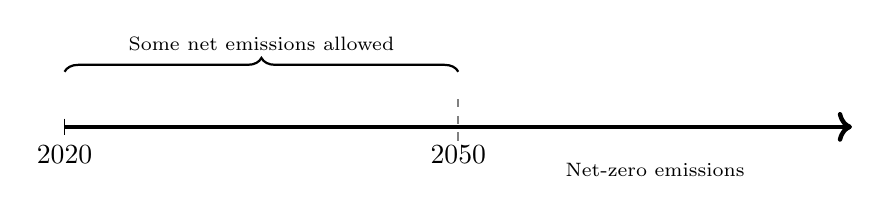
\begin{tikzpicture}
			\draw[ultra thick, ->] (0,0) -- (10,0);
			\foreach \x in {0}
			\draw (\x cm,3pt) -- (\x cm,-3pt);
			\foreach \x in {5}
			\draw[dashed, gray, thick] (\x cm,10pt) -- (\x cm,-6pt);
			% draw node
			\draw[thick] (0,0) node[below=3pt,thick] {2020} node[above=3pt] {};
			\draw[thick] (5,0) node[below=3pt,thick] {2050} node[above=3pt] {};
			\draw [thick ,decorate,decoration={brace,amplitude=5pt}] (0,0.7)  -- +(5,0) 
			node [black,midway,above=4pt, font=\scriptsize] {Some net emissions allowed};
			\node[draw=none, black, above=4pt, font=\scriptsize] (B1) at (7.5,-.9) {Net-zero emissions};
			
		\end{tikzpicture}
	}
	%	\pause
	%	\begin{center}
		%		\begin{figure}
			%	\caption{US CO$_2$ emission limit in Gt}
			%	\vspace{-2mm}
			%	\includegraphics[width=0.4\textwidth]{../codding_model/own_basedOnFried/optimalPol_010922_revision/figures/all_13Sept22_Tplus30/Emnet_goals_o0_lgd0.png}
			%\end{figure}
			%	\end{center}
	\end{frame}
	
	
	\begin{frame}{Preview of results}
		\centering
		\vspace{-3mm}
		\begin{itemize}[<+-| alert@+>]
			\setbeamercolor{alerted text}{} %change the font color
			\setbeamerfont{alerted text}{}
			%begin{minipage}[]{1\textwidth}
			%\begin{itemize}
			\item A combination of carbon and labor income taxes is optimal to target the allocation of research
			\vspace{3mm}
			\item Before the net-zero emission limit (ca. 2020-2050): 
			\begin{itemize}
				\item[-] lower carbon tax to maintain some fossil research %\tr{give an example of knowledge spillovers here}
				\item[-] a tax on labor income reduces emissions
			\end{itemize}
			\vspace{3mm}
			\item Under the net-zero emission limit (from 2050 onward): 
			\begin{itemize}
				\item[-]  higher carbon tax to foster green research
				\item[-]  a smaller tax on labor income boosts output
			\end{itemize}
			\vspace{3mm}
			\item Limited use of labor income tax \ar look at research subsidies
			%		\begin{itemize}
				%			\item[-] income tax remains beneficial to correct labor market distortions arising from lack of lump-sum rebates of carbon tax revenues
				%			%\item[-] when only green research subsidies are available, welfare smaller than with lump-sum rebates			
				%		\end{itemize}
			%; \tr{e.g. a higher marginal value of leisure}	%	\end{minipage}
	\end{itemize}
\end{frame}}

\begin{comment}
	\begin{frame}
		\begin{itemize}
			\item How to best implement emission targets in line with climate goals?
			\item 2 adjustment possibilities to reduce emissions: 
			\begin{enumerate}
				\item shift from fossil to green production technologies (e.g. carbon tax, green subsidies)
				\item lower the level of production overall (e.g. labor income taxes)
			\end{enumerate}
			\item Literature focuses on 1st point
		\end{itemize}
	\end{frame}
\end{comment}


\begin{frame}{Contribution to the literature}
	\begin{itemize}[<+->]
		\item \alert{\textbf{Standard to have inelastic labor supply in environmental policy discussion}}\\  \footnotesize{ \citep{Acemoglu2012TheChange, Golosov2014OptimalEquilibrium, Acemoglu2016TransitionTechnology, Fried2018ClimateAnalysis, Hart2019TheEconomists}}
		\\  \normalsize{\alert{\ar precludes studying combinations of policies targeted at the composition and\\ \hspace{5mm} the level of production }}
		\vspace{2mm}
		\item {Labor income taxes and environmental policies in the literature}
		\begin{itemize}
			\item[-]  government funding condition%; labor income tax generally passive 
		
			\footnotesize{ \citep{ LansBovenberg1994EnvironmentalTaxation, Goulder1995EnvironmentalGuide, Barrage2019OptimalPolicy}} % Not an env. policy instrument
			\item[-] {income inequality} % motivates taxing labor income as environmental policy tool 
		
			\footnotesize{\citep{Jacobs2019RedistributionCurves, Dobkowitz2022, Douenne2022OptimalHouseholds}}
			%	\item[-] This paper: novel motive for the use of labor income taxes within the optimal environmental policy: endogeneity of the allocation of researchers
		\end{itemize}		
		% Das klingt gut (differenzierung zwischen wirkungsweisen und nicht instrumenten! ): weil instrumente beide effekte haben können, dass die carbon tax auch das level beeinflusst wird ausgeklammert
		% I argue that we should study optimal env. policies allowing for level adjustments of production! I provide am example scenario where adjusting the level becomes part of the optimal policy
		\vspace{2mm}
		\item \alert{This paper}: classical trade-off between externality reduction and output% alone %directly % is optimal due to  directed technical change % and (ii) lack of research subsidies
		%	\footnotesize{\citep{Acemoglu2012TheChange}}
		%\\ \normalsize{\alert{\ar role for labor income taxation}}
		% weak double dividend literature (advantage to use env tac revenues to lower existing distortions; deviation of optimal env tax from pigou)
		%			\begin{itemize}
			%			%	\item[-] Research subsidies essential to implement first best.
			%			%	Otherwise, carbon tax higher to bolster green research; costly in terms of output
			%			%	\item[-]  In this case, labor income taxes may help get closer to first best
			%				\item[-] I add a richer, quantitative framework \ar new qualitative insights % increasing carbon tax, potentially fossil subsidy optimal
			%				\item[-]  insights on importance of additional measures
			%			\end{itemize}
		%	With knowledge spillovers \ar (i) increasing policy intervention, (ii) potentially advantageous to maintain some fossil research
		%	\vspace{2mm}
		%	% theirs is an analytical model; qualitative results; I look at a quantitative framework
		%	\item Quantitative framework builds on \cite{Fried2018ClimateAnalysis} %\ar new qualitative insights
		%	\begin{itemize}
			%		\item[-] I add a \alert{dynamic optimal policy analysis} under an exogenous \alert{dynamic emission target} %eventually declining to \alert{net-zero emissions}
			%		\item[-] \alert{elastic labor supply}
			%	\end{itemize}
	\end{itemize}
\end{frame}
%\begin{frame}{Mechanism}
%\begin{itemize}
%	\item in theory: optimal carbon tax set so that emitters internalize social costs of emissions
%	\vspace{2mm}
%	\item but, without research subsidy, carbon tax also used to target the direction of research
%	\vspace{2mm}
%	\item \normalsize{causes distortions on the labor market:}\\ households do not correctly internalize the social costs of labor
%\end{itemize}
%%\item<+->  \alert{sizable effect of skill heterogeneity}: \\ with only one skill, the optimal income tax increases social welfare by 0.85\%
%
%\end{frame}
\begin{frame}{Outline}
	\tableofcontents
\end{frame}

\section{Model}
\begin{frame}{Model}
	\begin{figure}[h]
		\vspace{-4mm}
		\centering
		\begin{tikzpicture}[auto,scale=.7, transform shape]
			\node[circll] (A) at (-7,4) {\textbf{{\hyperlink{prodmod}{Production}}}\\ \textbf{{and Research}}};
			\node[circll] (B) at (7,4) {\textbf{{{Representative}}}\\ \textbf{{{Household}}}};
			\node[circll] (D) at (0,9) {\textbf{{Government}} }; 
			\node[draw=none] (B1) at (5,4.25) {};
			\node[draw=none] (B2) at (5,3.5) {};
			\node[draw=none] (BA1) at (-5,4.25) {};
			\node[draw=none] (BA2) at (-5,3.5) {};
			\node[draw=none] (D1) at (1.8,7.8) {};
			
			\node[draw=none] (B22) at (6.4,5.6) {};
			\node[draw=none] (D2) at (2.3,8.5) {};
			\node[draw=none] (B3) at (5.3,5.3) {};
			\node[draw=none] (D3) at (-1.5,7) {};
			\node[draw=none] (A1) at (-4.2,4.6) {};
			\node[draw=none] (D4) at (-2,8.3) {};
			\node[draw=none] (A4) at (-6,5.4) {};
			\draw [draw=none] (B22) to node[pos=0.65, swap]{\textcolor{black!1}{Tax on labor, $\pmb{\tau_{\iota}}$:}} (D2);
			\draw [draw=none] (B22) to node[pos=0.45, swap]{\textcolor{black!1}{$\pmb{\tau_{\iota}} \uparrow$:  labor supply $\downarrow$ \ar emissions $\downarrow$}} (D2);
			\draw [draw=none] (B22) to node[pos=0.3, swap]{\textcolor{black!1}{$\pmb{\tau_{\iota}} \downarrow$:    labor supply $\uparrow$ \ar output $\uparrow$}} (D2);
			\draw [draw=none] (D1) to node[pos=0.5, swap]{\textcolor{black!1}{Transfers}} (B3);
			
			\draw [draw=none] (B1) to node[pos=0.75, swap]{\textcolor{black!1}{Workers and scientists}} (BA1);
			\draw [draw=none] (BA2) to node[pos=0.75, swap]{\textcolor{black!1}{Final good}} (B2);
			%	\draw [->] (A4) to node[pos=0.5, swap]{\alert{Tax on carbon, $\pmb{\tau_F}$}}   (D4);
		\end{tikzpicture}
	\end{figure}
\end{frame}


\addtocounter{framenumber}{-1}
\begin{frame}{Model}
	\begin{figure}[h]
		\vspace{-4mm}
		\centering
		\begin{tikzpicture}[auto,scale=.7, transform shape]
			\node[circll] (A) at (-7,4) {\textbf{{\hyperlink{prodmod}{Production}}}\\ \textbf{{and Research}}};
			\node[circll] (B) at (7,4) {\textbf{{\alert{Representative}}}\\ \textbf{{\alert{Household}}}};
			\node[circll] (D) at (0,9) {\textbf{{Government}} }; 
			\node[draw=none] (B1) at (5,4.25) {};
			\node[draw=none] (B2) at (5,3.5) {};
			\node[draw=none] (BA1) at (-5,4.25) {};
			\node[draw=none] (BA2) at (-5,3.5) {};
			\node[draw=none] (D1) at (1.8,7.8) {};
			
			\node[draw=none] (B22) at (6.4,5.6) {};
			\node[draw=none] (D2) at (2.3,8.5) {};
			\node[draw=none] (B3) at (5.3,5.3) {};
			\node[draw=none] (D3) at (-1.5,7) {};
			\node[draw=none] (A1) at (-4.2,4.6) {};
			\node[draw=none] (D4) at (-2,8.3) {};
			\node[draw=none] (A4) at (-6,5.4) {};
			\draw [draw=none] (B22) to node[pos=0.65, swap]{\textcolor{black!1}{Tax on labor, $\pmb{\tau_{\iota}}$:}} (D2);
			\draw [draw=none] (B22) to node[pos=0.45, swap]{\textcolor{black!1}{$\pmb{\tau_{\iota}} \uparrow$:  labor supply $\downarrow$ \ar emissions $\downarrow$}} (D2);
			\draw [draw=none] (B22) to node[pos=0.3, swap]{\textcolor{black!1}{$\pmb{\tau_{\iota}} \downarrow$:    labor supply $\uparrow$ \ar output $\uparrow$}} (D2);
			\draw [draw=none] (D1) to node[pos=0.5, swap]{\textcolor{black!1}{Transfers}} (B3);
			
			\draw [draw=none] (B1) to node[pos=0.75, swap]{\textcolor{black!1}{Workers and scientists}} (BA1);
			\draw [draw=none] (BA2) to node[pos=0.75, swap]{\textcolor{black!1}{Final good}} (B2);
			%	\draw [->] (A4) to node[pos=0.5, swap]{\alert{Tax on carbon, $\pmb{\tau_F}$}}   (D4);
		\end{tikzpicture}
	\end{figure}
\end{frame}


\addtocounter{framenumber}{-1}
\begin{frame}{Model}
	\begin{figure}[h]
		\vspace{-4mm}
		\centering
		\begin{tikzpicture}[auto,scale=.7, transform shape]
			\node[circll] (A) at (-7,4) {\textbf{{\hyperlink{prodmod}{Production}}}\\ \textbf{{and Research}}};
			\node[circll] (B) at (7,4) {\textbf{{{Representative}}}\\ \textbf{{{Household}}}};
			\node[circll] (D) at (0,9) {\textbf{{Government}} }; 
			\node[draw=none] (B1) at (5,4.25) {};
			\node[draw=none] (B2) at (5,3.5) {};
			\node[draw=none] (BA1) at (-5,4.25) {};
			\node[draw=none] (BA2) at (-5,3.5) {};
			\node[draw=none] (D1) at (1.8,7.8) {};
			
			\node[draw=none] (B22) at (6.4,5.6) {};
			\node[draw=none] (D2) at (2.3,8.5) {};
			\node[draw=none] (B3) at (5.3,5.3) {};
			\node[draw=none] (D3) at (-1.5,7) {};
			\node[draw=none] (A1) at (-4.2,4.6) {};
			\node[draw=none] (D4) at (-2,8.3) {};
			\node[draw=none] (A4) at (-6,5.4) {};
			\draw [draw=none] (B22) to node[pos=0.65, swap]{\textcolor{black!1}{Tax on labor, $\pmb{\tau_{\iota}}$:}} (D2);
			\draw [draw=none] (B22) to node[pos=0.45, swap]{\textcolor{black!1}{$\pmb{\tau_{\iota}} \uparrow$:  labor supply $\downarrow$ \ar emissions $\downarrow$}} (D2);
			\draw [draw=none] (B22) to node[pos=0.3, swap]{\textcolor{black!1}{$\pmb{\tau_{\iota}} \downarrow$:    labor supply $\uparrow$ \ar output $\uparrow$}} (D2);
			\draw [draw=none] (D1) to node[pos=0.5, swap]{\textcolor{black!1}{Transfers}} (B3);
			
			\draw [->] (B1) to node[pos=0.75, swap]{Workers and scientists} (BA1);
			\draw [->] (BA2) to node[pos=0.75, swap]{Final good} (B2);
			%	\draw [->] (A4) to node[pos=0.5, swap]{\alert{Tax on carbon, $\pmb{\tau_F}$}}   (D4);
		\end{tikzpicture}
	\end{figure}
\end{frame}
\addtocounter{framenumber}{-1}
\begin{frame}{Model}
	\begin{figure}[h]
		\vspace{-4mm}
		\centering
		\begin{tikzpicture}[auto,scale=.7, transform shape]
			\node[circll] (A) at (-7,4) {\textbf{{\hyperlink{prodmod}{Production}}}\\ \textbf{{and Research}}};
			\node[circll] (B) at (7,4) {\textbf{{{Representative}}}\\ \textbf{{{Household}}}};
			\node[circll] (D) at (0,9) {\textbf{{Government}} }; 
			\node[draw=none] (B1) at (5,4.25) {};
			\node[draw=none] (B2) at (5,3.5) {};
			\node[draw=none] (BA1) at (-5,4.25) {};
			\node[draw=none] (BA2) at (-5,3.5) {};
			\node[draw=none] (D1) at (1.8,7.8) {};
			
			\node[draw=none] (B22) at (6.4,5.6) {};
			\node[draw=none] (D2) at (2.3,8.5) {};
			\node[draw=none] (B3) at (5.3,5.3) {};
			\node[draw=none] (D3) at (-1.5,7) {};
			\node[draw=none] (A1) at (-4.2,4.6) {};
			\node[draw=none] (D4) at (-2,8.3) {};
			\node[draw=none] (A4) at (-6,5.4) {};
			\draw [->] (B22) to node[pos=0.65, swap]{{Tax on labor, $\pmb{\tau_{\iota}}$}\textcolor{black!1}{:}} (D2);
			\draw [draw=none] (B22) to node[pos=0.45, swap]{\textcolor{black!1}{$\pmb{\tau_{\iota}} \uparrow$:  labor supply $\downarrow$ \ar emissions $\downarrow$}} (D2);
			\draw [draw=none] (B22) to node[pos=0.3, swap]{\textcolor{black!1}{$\pmb{\tau_{\iota}} \downarrow$:    labor supply $\uparrow$ \ar output $\uparrow$}} (D2);
			\draw [->] (D1) to node[pos=0.5, swap]{Transfers} (B3);
			
			\draw [->] (B1) to node[pos=0.75, swap]{Workers and scientists} (BA1);
			\draw [->] (BA2) to node[pos=0.75, swap]{Final good} (B2);
			%	\draw [->] (A4) to node[pos=0.5, swap]{\alert{Tax on carbon, $\pmb{\tau_F}$}}   (D4);
		\end{tikzpicture}
	\end{figure}
\end{frame}

\addtocounter{framenumber}{-1}
\begin{frame}{Model}
	\begin{figure}[h]
		\vspace{-4mm}
		\centering
		\begin{tikzpicture}[auto,scale=.7, transform shape]
			\node[circll] (A) at (-7,4) {\textbf{{\hyperlink{prodmod}{Production}}}\\ \textbf{{and Research}}};
			\node[circll] (B) at (7,4) {\textbf{{{Representative}}}\\ \textbf{{{Household}}}};
			\node[circll] (D) at (0,9) {\textbf{{Government}} }; 
			\node[draw=none] (B1) at (5,4.25) {};
			\node[draw=none] (B2) at (5,3.5) {};
			\node[draw=none] (BA1) at (-5,4.25) {};
			\node[draw=none] (BA2) at (-5,3.5) {};
			\node[draw=none] (D1) at (1.8,7.8) {};
			
			\node[draw=none] (B22) at (6.4,5.6) {};
			\node[draw=none] (D2) at (2.3,8.5) {};
			\node[draw=none] (B3) at (5.3,5.3) {};
			\node[draw=none] (D3) at (-1.5,7) {};
			\node[draw=none] (A1) at (-4.2,4.6) {};
			\node[draw=none] (D4) at (-2,8.3) {};
			\node[draw=none] (A4) at (-6,5.4) {};
			\draw [->] (B22) to node[pos=0.65, swap]{\alert{Tax on labor, $\pmb{\tau_{\iota}}$:}} (D2);
			\draw [draw=none] (B22) to node[pos=0.45, swap]{\alert{$\pmb{\tau_{\iota}} \uparrow$:  labor supply $\downarrow$ \ar emissions $\downarrow$}} (D2);
			\draw [draw=none] (B22) to node[pos=0.3, swap]{\textcolor{black!1}{$\pmb{\tau_{\iota}} \downarrow$:    labor supply $\uparrow$ \ar output $\uparrow$}} (D2);
			\draw [->] (D1) to node[pos=0.5, swap]{Transfers} (B3);
			
			\draw [->] (B1) to node[pos=0.75, swap]{Workers and scientists} (BA1);
			\draw [->] (BA2) to node[pos=0.75, swap]{Final good} (B2);
			%	\draw [->] (A4) to node[pos=0.5, swap]{\alert{Tax on carbon, $\pmb{\tau_F}$}}   (D4);
		\end{tikzpicture}
	\end{figure}
\end{frame}
\addtocounter{framenumber}{-1}
\begin{frame}{Model}
	\begin{figure}[h]
		\vspace{-4mm}
		\centering
		\begin{tikzpicture}[auto,scale=.7, transform shape]
			\node[circll] (A) at (-7,4) {\textbf{{\hyperlink{prodmod}{Production}}}\\ \textbf{{and Research}}};
			\node[circll] (B) at (7,4) {\textbf{{{Representative}}}\\ \textbf{{{Household}}}};
			\node[circll] (D) at (0,9) {\textbf{{Government}} }; 
			\node[draw=none] (B1) at (5,4.25) {};
			\node[draw=none] (B2) at (5,3.5) {};
			\node[draw=none] (BA1) at (-5,4.25) {};
			\node[draw=none] (BA2) at (-5,3.5) {};
			\node[draw=none] (D1) at (1.8,7.8) {};
			
			\node[draw=none] (B22) at (6.4,5.6) {};
			\node[draw=none] (D2) at (2.3,8.5) {};
			\node[draw=none] (B3) at (5.3,5.3) {};
			\node[draw=none] (D3) at (-1.5,7) {};
			\node[draw=none] (A1) at (-4.2,4.6) {};
			\node[draw=none] (D4) at (-2,8.3) {};
			\node[draw=none] (A4) at (-6,5.4) {};
			\draw [->] (B22) to node[pos=0.65, swap]{\alert{Tax on labor, $\pmb{\tau_{\iota}}$:}} (D2);
			\draw [draw=none] (B22) to node[pos=0.45, swap]{\alert{$\pmb{\tau_{\iota}} \uparrow$:  labor supply $\downarrow$ \ar emissions $\downarrow$}} (D2);
			\draw [draw=none] (B22) to node[pos=0.3, swap]{\alert{$\pmb{\tau_{\iota}} \downarrow$:    labor supply $\uparrow$ \ar output $\uparrow$}} (D2);
			\draw [->] (D1) to node[pos=0.5, swap]{Transfers} (B3);
			
			\draw [->] (B1) to node[pos=0.75, swap]{Workers and scientists} (BA1);
			\draw [->] (BA2) to node[pos=0.75, swap]{Final good} (B2);
			%	\draw [->] (A4) to node[pos=0.5, swap]{\alert{Tax on carbon, $\pmb{\tau_F}$}}   (D4);
		\end{tikzpicture}
	\end{figure}
\end{frame}




\begin{frame}{Representative household}
	\hypertarget{backhh}{}
	%\text{\textbf{Householdrt}}
	\vspace{2mm}
	\begin{minipage}[t!]{1\textwidth}
		\begin{align*}
			%	\tikzmarkin{first0}(1.5,2.7)(-1.2,-2.5)
			%	\underset{c_{s,i},c_{n,i}, l_i}{\max} \ \hspace{2mm} U(c_{s,i}, c_{n,i}, l_i; h_n)= 
			\max_{\{C_t\}^\infty_{t=0}, \{H_{t}\}^\infty_{t=0}, \{S_{t}\}^\infty_{t=0}} \sum_{t=0}^{\infty}\beta^t\left(\log(C_t)-\chi\frac{H_{t}^{1+\sigma}}{1+\sigma}-\chi_s\frac{S_{t}^{1+\sigma}}{1+\sigma}\right)
			\\
			\vspace{4mm}
			\\
			\text{s.t.}\ C_t=\lambda_t\left(w_{t}H_{t}\right)^{(\alert{\pmb{1-\tau_{\iota t}}})}+\lambda_t \left(w_{st}S_t\right)^{(\alert{\pmb{1-\tau_{\iota t}}})}+T_t%+Gov_t
			%\\
			%\hspace{2mm}\ H_{t}\leq \bar{H}; \hspace{4mm} S_{t}\leq \bar{H}
			%	\tikzmarkend{first0}
		\end{align*}
	\end{minipage}
	
	\small
	\vspace{4mm}
	\hspace{-8mm}
	\begin{minipage}[t!]{0.26\textwidth}
		\vspace{8mm}
		\begin{itemize}
			\item[] $C_{t}$: consumption\vspace{-2mm}
			\item[] $H_{t}$: hours workers\vspace{-2mm}
			\item[] $S_{t}$: hours scientists\vspace{-2mm}
			\item[] $w_{t}$: wage workers %\vspace{-2mm}
		\end{itemize}
	\end{minipage}
	\begin{minipage}[t!]{0.37\textwidth}
		\vspace{8mm}
		\begin{itemize}
			\item[] $w_{st}$: wage scientists  \vspace{-2mm}
			\item[] $\lambda_{t}$: scale income tax scheme  \vspace{-2mm}
			\item[] $\tau_{\iota t}$: income tax progressivity 	\vspace{-2mm}	
			\item[] $T_{t}$: government transfers
		\end{itemize}
	\end{minipage}
	\begin{minipage}[t!]{0.39\textwidth}
		\vspace{8mm}
		\begin{itemize}
			\item[] $\sigma$: curvature disutility of labor  \vspace{-2mm}
			\item[] $\chi$: disutility of work
			\vspace{-2mm}	
			\item[] $\chi_s$: disutility of research
			\vspace{-2mm}	
			\item[] $ \beta$: discount factor  %\vspace{-2mm}
		\end{itemize}
	\end{minipage}
	
\end{frame}

%
%\begin{frame}{Model}
%	\begin{figure}[h]
	%		\vspace{-4mm}
	%		\centering
	%		\begin{tikzpicture}[auto,scale=.7, transform shape]
		%			\node[circll] (A) at (-7,4) {\textbf{{\alert{Production}}}\\ \alert{\textbf{{and Research}}}};
		%			\node[circll] (B) at (7,4) {\textbf{\hyperlink{backhh}{{Representative}}}\\ \textbf{\hyperlink{backhh}{{Household}}}};
		%			\node[circll] (D) at (0,9) {\textbf{{Government}} }; 
		%			\node[draw=none] (B1) at (5,4.25) {};
		%			\node[draw=none] (B2) at (5,3.5) {};
		%			\node[draw=none] (BA1) at (-5,4.25) {};
		%			\node[draw=none] (BA2) at (-5,3.5) {};
		%			\node[draw=none] (D1) at (1.8,7.8) {};
		%			
		%			\node[draw=none] (B22) at (6.4,5.6) {};
		%			\node[draw=none] (D2) at (2.3,8.5) {};
		%			\node[draw=none] (B3) at (5.3,5.3) {};
		%			\node[draw=none] (D3) at (-1.5,7) {};
		%			\node[draw=none] (A1) at (-4.2,4.6) {};
		%			\node[draw=none] (D4) at (-2,8.3) {};
		%			\node[draw=none] (A4) at (-6,5.4) {};
		%			%			\draw [->] (B22) to node[pos=0.5, swap]{{Tax on labor, $\pmb{\tau_{\iota}}$}} (D2);
		%			%			\draw [->] (D1) to node[pos=0.5, swap]{Transfers} (B3);
		%			
		%%			\draw [->] (B1) to node[pos=0.75, swap]{Workers and scientists} (BA1);
		%%			\draw [->] (BA2) to node[pos=0.75, swap]{Final good} (B2);
		%%			\draw [->] (A4) to node[pos=0.5, swap]{\alert{Tax on carbon, $\pmb{\tau_F}$}}   (D4);
		%		\end{tikzpicture}
	%		
	%	\end{figure}
%\end{frame}
%\addtocounter{framenumber}{-1}
\begin{frame}{Model}
	\begin{figure}[h]
		\vspace{-4mm}
		\centering
		\begin{tikzpicture}[auto,scale=.7, transform shape]
			\node[circll] (A) at (-7,4) {\textbf{{\alert{Production}}}\\ \alert{\textbf{{and Research}}}};
			\node[circll] (B) at (7,4) {\textbf{\hyperlink{backhh}{{Representative}}}\\ \textbf{\hyperlink{backhh}{{Household}}}};
			\node[circll] (D) at (0,9) {\textbf{{Government}} }; 
			\node[draw=none] (B1) at (5,4.25) {};
			\node[draw=none] (B2) at (5,3.5) {};
			\node[draw=none] (BA1) at (-5,4.25) {};
			\node[draw=none] (BA2) at (-5,3.5) {};
			\node[draw=none] (D1) at (1.8,7.8) {};
			
			\node[draw=none] (B22) at (6.4,5.6) {};
			\node[draw=none] (D2) at (2.3,8.5) {};
			\node[draw=none] (B3) at (5.3,5.3) {};
			\node[draw=none] (D3) at (-1.5,7) {};
			\node[draw=none] (A1) at (-4.2,4.6) {};
			\node[draw=none] (D4) at (-2,8.3) {};
			\node[draw=none] (A4) at (-6,5.4) {};
			%			\draw [->] (B22) to node[pos=0.5, swap]{{Tax on labor, $\pmb{\tau_{\iota}}$}} (D2);
			%			\draw [->] (D1) to node[pos=0.5, swap]{Transfers} (B3);
			
			\draw [->] (B1) to node[pos=0.75, swap]{Workers and scientists} (BA1);
			\draw [->] (BA2) to node[pos=0.75, swap]{Final good} (B2);
			%\draw [->] (A4) to node[pos=0.5, swap]{\alert{Tax on carbon, $\pmb{\tau_F}$}}   (D4);
		\end{tikzpicture}
		
	\end{figure}
\end{frame}


\addtocounter{framenumber}{-1}
\begin{frame}{Model}
	\begin{figure}[h]
		\vspace{-4mm}
		\centering
		\begin{tikzpicture}[auto,scale=.7, transform shape]
			\node[circll] (A) at (-7,4) {\textbf{{\hyperlink{prodmod}{Production}}}\\ \textbf{{and Research}}};
			\node[circll] (B) at (7,4) {\textbf{\hyperlink{backhh}{{Representative}}}\\ \textbf{\hyperlink{backhh}{{Household}}}};
			\node[circll] (D) at (0,9) {\textbf{{Government}} }; 
			\node[draw=none] (B1) at (5,4.25) {};
			\node[draw=none] (B2) at (5,3.5) {};
			\node[draw=none] (BA1) at (-5,4.25) {};
			\node[draw=none] (BA2) at (-5,3.5) {};
			\node[draw=none] (D1) at (1.8,7.8) {};
			
			\node[draw=none] (B22) at (6.4,5.6) {};
			\node[draw=none] (D2) at (2.3,8.5) {};
			\node[draw=none] (B3) at (5.3,5.3) {};
			\node[draw=none] (D3) at (-1.5,7) {};
			\node[draw=none] (A1) at (-4.2,4.6) {};
			\node[draw=none] (D4) at (-2,8.3) {};
			\node[draw=none] (A4) at (-6,5.4) {};
			%			\draw [->] (B22) to node[pos=0.5, swap]{{Tax on labor, $\pmb{\tau_{\iota}}$}} (D2);
			%			\draw [->] (D1) to node[pos=0.5, swap]{Transfers} (B3);
			
			\draw [->] (B1) to node[pos=0.75, swap]{Workers and scientists} (BA1);
			\draw [->] (BA2) to node[pos=0.75, swap]{Final good} (B2);
			\draw [->] (A4) to node[pos=0.5, swap]{\alert{Tax on carbon, $\pmb{\tau_F}$}}   (D4);
		\end{tikzpicture}
		
	\end{figure}
\end{frame}

\begin{comment}
	\begin{frame}{Production}
		\begin{figure}[h]
			\vspace{-10mm}
			\centering
			\begin{tikzpicture}[auto,scale=.7, transform shape]
				\node[circll] (A) at (0,17) {\textbf{Final}\textbf{ Good}}; 
				\node[circll] (B) at (-6,14) {\textbf{Energy}};
				\node[circll] (C) at (5,12) {\textbf{{Non-energy}}};
				\node[circll] (D) at (-10,12) {\textbf{{Fossil}}};
				\node[circll] (E) at (-2,12) {\textbf{{Green}}};
				\node[sphere] (Ems) at (-11,16) {\textbf{Emissions}};
				
				%		\node[circllsmall] (CM) at (4.6,8) {\textbf{{Machines}}};
				%		\node[circllsmall] (CL) at (7.4,8) {\textbf{{Labor}}};			\node[circllsmall] (EM) at (-3.4,8) {\textbf{{Machines}}};
				%	    \node[circllsmall] (EL) at (-0.6,8) {\textbf{{Labor}}};
				%	    \node[circllsmall] (DM) at (-11.4,8) {\textbf{{Machines}}};
				%	    \node[circllsmall] (DL) at (-8.6,8) {\textbf{{Labor}}};
				
				
				\draw [->] (B) to node[pos=0.5, swap]{} (A);
				\draw [->] (C) to node[pos=0.5, swap]{} (A);
				
				\draw [->] (E) to node[pos=0.5, swap]{} (B);
				\draw [->] (D) to node[pos=0.5, swap]{} (B);
				\draw [->] (D) to node[pos=0.5, swap]{} (Ems);
			\end{tikzpicture}
			
		\end{figure}
	\end{frame}
	content...
\end{comment}

\begin{frame}{Production: final and energy good}
	\vspace{-10mm}
	\hypertarget{prodmod}{}
	\begin{align*}
		%		\tikzmarkin{first}(1.3,1.2)(-1,-0.8)
		\text{Final good}\hspace{4mm}&Y_t =\left(\delta_y^{\frac{1}{\varepsilon_y}}E_t^\frac{\varepsilon_y-1}{\varepsilon_y}+(1-\delta_y)^{\frac{1}{\varepsilon_y}}N_t^\frac{\varepsilon_y-1}{\varepsilon_y}\right)^\frac{\varepsilon_y}{\varepsilon_y-1} \\
		\ \\
		\text{Energy}\hspace{4mm}&E_t =\left({F}_t^\frac{\varepsilon_e-1}{\varepsilon_e}+G_t^\frac{\varepsilon_e-1}{\varepsilon_e}\right)^\frac{\varepsilon_e}{\varepsilon_e-1}\\
		\ \\
		\text{Demand energy producers}\hspace{4mm}&\frac{F_t}{G_t} = \left(\frac{p_{Gt}}{p_{Ft}+\alert{\pmb{\tau_{Ft}}}}\right)^{\varepsilon_e}
		%	\tikzmarkend{third}
	\end{align*}
	
	\small
	\vspace{4mm}
	\hspace{-4mm}
	\begin{minipage}[t!]{0.24\textwidth}
		\vspace{0mm}
		\begin{itemize}	
			\item[]$F_t$: fossil energy
			\vspace{-2mm}	
			\item[]$G_t$: green energy
			\vspace{-7mm}	
			\item[]$N_t$: non-energy
		\end{itemize}
	\end{minipage}
	\begin{minipage}[t!]{0.24\textwidth}
		\vspace{0mm}
		\begin{itemize}
			\item[] $p_{Gt}$: price green  \vspace{-2mm}
			\item[] $p_{Ft}$: price fossil
			\vspace{-2mm}	
			\item[] $\tau_{Ft}$: carbon tax
		\end{itemize}
	\end{minipage}
	\begin{minipage}[t!]{0.47\textwidth}
		\vspace{0mm}
		\begin{itemize}
			\item[] $\delta_{y}$: weight on energy\vspace{-2mm}
			\item[] $\varepsilon_y$: elasticity of substitution $E_t$ and $N_t$ \vspace{-2mm}
			\item[] $\varepsilon_e$: elasticity of substitution $F_t$ and $G_t$
		\end{itemize}
	\end{minipage}
\end{frame}

%\addtocounter{framenumber}{-1}
\begin{frame}{Production: intermediate goods $J\in \{N,F,G\}$ }
	\vspace{0mm}
	%Competitive producers
	\begin{align*}
		\underset{\{x_{Jit}\}_{i=0}^1, L_{Jt}}{\max}\ & p_{Jt}J_t-w_{t}L_{Jt}-\int_{0}^{1}p_{xJit}x_{Jit}di \\ \ \\
		\text{s.t.}\ & J_{t}=L_{Jt}^{1-\alpha_J}\int_{0}^{1}A^{1-\alpha_J}_{Jit}x_{Jit}^{\alpha_J}di
	\end{align*}
	
	\small
	\vspace{10mm}
	\hspace{-4mm}
	\begin{minipage}[t!]{0.3\textwidth}
		\vspace{0mm}
		\begin{itemize}	
			\item[]$L_{Jt}\ $: labor 
			\vspace{-2mm}	
			\item[]$x_{Jit}\ $: machines 
			\vspace{-2mm}	
			\item[]$p_{xJit}$: price machine 
		\end{itemize}
	\end{minipage}
	\begin{minipage}[t!]{0.5\textwidth}
		\vspace{0mm}
		\begin{itemize}
			\item[] $A_{Jit}$: productivity machine $i$ sector $J$ \vspace{-2mm}
			\item[] $J$\ \  : sector N(on-energy),F(ossil),G(reen)
			\vspace{-2mm}	
			\item[] $\alpha_J$\ : capital share 
		\end{itemize}
	\end{minipage}
\end{frame}

\begin{frame}{Production: machines and innovation}
	\vspace{-8mm}
	\begin{align*}
		%	\tikzmarkin{sixth}(6.3,4)(-2.7,-3.8)
		\underset{p_{xJit}, s_{Jit}}{\max}\ & p_{xJit}(1+\zeta_{J})x_{Jit}-x_{Jit}-w_{st}s_{Jit}
		\\ 
		\text{s.t.}\ &(1)\ x_{Jit}=\left(\frac{\alpha_Jp_{Jt}}{p_{xJit}}\right)^{\frac{1}{1-\alpha_J}}L_{Jt}A_{Jit}\\ \ \\ %x_{ijt}= \left(\frac{p_{ft}(1-\tau_{jt})\alpha_j}{p_{xijt}}\right)^\frac{1}{1-\alpha_j}A_{ijt}L_{jt}\\
		& (2)\ A_{Jit}=f_{Jt}(s_{Jit})%A_{Jt-1}\left(1+\gamma\left(\frac{s_{Jit}}{\rho_J}\right)^\eta\left(\frac{A_{t-1}}{A_{Jt-1}}\right)^\phi\right)
		%	\tikzmarkend{sixth}
	\end{align*}
	
	\small
	\vspace{4mm}
	\hspace{-4mm}	\begin{minipage}[t!]{0.32\textwidth}
		\vspace{-1mm}
		\begin{itemize}
			\item[-] monopolistic competition 
			\vspace{-4mm}
			\item[] \ 
		\end{itemize}	
	\end{minipage}
	\begin{minipage}[t!]{0.5\textwidth}
		\vspace{0mm}
		\begin{itemize}	
			\item[]$\zeta_{J}$: subsidy
			\vspace{-2mm}	
			\item[]$s_{Jit}$: scientists
			\vspace{-2mm}	
			\item[]$A_{Jit}$: productivity machine $i$ sector $J$
		\end{itemize}
	\end{minipage}
	%\begin{minipage}[t!]{0.32\textwidth}
	%	\vspace{0mm}
	%	\begin{itemize}
		%		\item[] $\eta$: returns to research  \vspace{-2mm}
		%		\item[] $\rho_j$: research processes
		%		\vspace{-2mm}	
		%		\item[] $\gamma$: productivity scientists
		%	\end{itemize}
	%\end{minipage}
\end{frame}

\begin{comment}
	\addtocounter{framenumber}{-1}
	\begin{frame}{Production: machines and innovation}
		\vspace{-2mm}
		Monopolistically competitive machine producer $i$ in sector $J$
		\begin{align*}
			%	\tikzmarkin{sixth}(6.3,4)(-2.7,-3.8)
			\underset{p_{xJit}, s_{Jit}}{\max}\ & p_{xJit}(1+\zeta_{Jt})x_{Jit}-x_{Jit}-w_{st}s_{Jit}
			\\ 
			s.t.\ &(1)\ x_{Jit}=\left(\alpha_Jp_{Jt}\right)^{\frac{1}{1-\alpha_J}}L_{Jt}A_{Jit}\\ \ \\ %x_{ijt}= \left(\frac{p_{ft}(1-\tau_{jt})\alpha_j}{p_{xijt}}\right)^\frac{1}{1-\alpha_j}A_{ijt}L_{jt}\\
			& (2)\ A_{Jit}=A_{Jt-1}\left(1+\gamma\left(\frac{s_{Jit}}{\rho_J}\right)^\eta\left(\frac{A_{t-1}}{A_{Jt-1}}\right)^\phi\right)
			%	\tikzmarkend{sixth}
		\end{align*}
		
		\small
		\vspace{4mm}
		\hspace{-4mm}
		\begin{minipage}[t!]{0.4\textwidth}
			\vspace{0mm}
			\begin{itemize}	
				\item[]$\zeta_{Jt}$: subsidy
				\vspace{-2mm}	
				\item[]$s_Ji$: scientists
				\vspace{-2mm}	
				\item[]$\phi$: knowledge spillovers
			\end{itemize}
		\end{minipage}
		\begin{minipage}[t!]{0.5\textwidth}
			\vspace{0mm}
			\begin{itemize}
				\item[] $\eta$: returns to research  \vspace{-2mm}
				\item[] $\rho_j$: research processes
				\vspace{-2mm}	
				\item[] $\gamma$: productivity scientists
			\end{itemize}
		\end{minipage}
	\end{frame}
	
	content...
\end{comment}

%\begin{frame}{In more detail}
%\begin{enumerate}
%	\item<1-> effect of carbon tax on the allocation of scientists
%	\item<2-> innovation
%\end{enumerate}
%\end{frame}


\begin{frame}{Innovation}
	\pause
	\vspace{-5mm}
	% talk about productivity of research bcs it determines optimal allocation of research
	\large
	\begin{align*}
		A_{Jit}={A_{Jt-1}}\left(1+\gamma{\left(\frac{s_{Jit}}{\rho_J}\right)^\eta}{\left(\frac{A_{t-1}}{A_{Jt-1}}\right)^\phi}\right)
	\end{align*}
	\normalsize
	\begin{enumerate}
		\item[]  \textcolor{black!1}{Within-sector knowledge spillovers} %: sector-specific knowledge renders scientists more productive} % \footnotesize{one-period patents} % due to patent structure not taken into account by machine producers when demanding research. 
	%		\begin{itemize}
		%	\item<+-> scientists in most advanced, fossil sector are more productive
		%			\item<+-> shift to green research early on to make green research more productive tomorrow
		%		\end{itemize}
	\item[] \textcolor{black!1}{Cross-sectoral knowledge spillovers} %knowledge from other sectors increases productivity of scientists
	\item[] \textcolor{black!1}{Inefficiencies  due to one-period patents}  % decreasing returns to research, $\eta<1$
\end{enumerate}
\small
\vspace{4mm}
\hspace{-2mm}
\begin{minipage}[t!]{0.43\textwidth}
	\vspace{0mm}
	\begin{itemize}
		\item[] $A_{Jt}$: sector-specific technology
		\vspace{-2mm}		
		\item[] $A_t$: aggregate technology
		\vspace{-2mm}
		\item[] $\gamma$ : productivity of scientists
	\end{itemize}
\end{minipage}
\vspace{-5mm}
\begin{minipage}[t!]{0.55\textwidth}
	\vspace{0mm}
	\begin{itemize}	
		\item[] $\rho_J$: number of research processes in sector $J$
		\vspace{-2mm}			
		\item[] $\eta$ : returns to research
		\vspace{-2mm}			
		\item[] $\phi$ : relative importance knowledge spillovers
	\end{itemize}
\end{minipage}
\end{frame}

\addtocounter{framenumber}{-1}
\begin{frame}{Innovation}

	\vspace{-5mm}
	% talk about productivity of research bcs it determines optimal allocation of research
	\large
	\begin{align*}
		A_{Jit}=\alert{A_{Jt-1}}\left(1+\gamma{\left(\frac{s_{Jit}}{\rho_J}\right)^\eta}{\left(\frac{A_{t-1}}{A_{Jt-1}}\right)^\phi}\right)
	\end{align*}
	\normalsize
	\begin{enumerate}
		\item \alert{Within-sector knowledge spillovers} %: sector-specific knowledge renders scientists more productive} % \footnotesize{one-period patents} % due to patent structure not taken into account by machine producers when demanding research. 
		%		\begin{itemize}
			%	\item<+-> scientists in most advanced, fossil sector are more productive
			%			\item<+-> shift to green research early on to make green research more productive tomorrow
			%		\end{itemize}
	\item[] \textcolor{black!1}{Cross-sectoral knowledge spillovers}
\item[] \textcolor{black!1}{Inefficiencies: one-period patents}
	\end{enumerate}
	\small
	\vspace{4mm}
	\hspace{-2mm}
	\begin{minipage}[t!]{0.43\textwidth}
		\vspace{0mm}
		\begin{itemize}
			\item[] $A_{Jt}$: sector-specific technology
			\vspace{-2mm}		
			\item[] $A_t$: aggregate technology
			\vspace{-2mm}
			\item[] $\gamma$ : productivity of scientists
		\end{itemize}
	\end{minipage}
	\vspace{-5mm}
	\begin{minipage}[t!]{0.55\textwidth}
		\vspace{0mm}
		\begin{itemize}	
			\item[] $\rho_J$: number of research processes in sector $J$
			\vspace{-2mm}			
			\item[] $\eta$ : returns to research
			\vspace{-2mm}			
			\item[] $\phi$ : relative importance knowledge spillovers
		\end{itemize}
	\end{minipage}
\end{frame}

\addtocounter{framenumber}{-1}
\begin{frame}{Innovation}
	\vspace{-5mm}
	\large
	\begin{align*}
		A_{Jit}={A_{Jt-1}}\left(1+\gamma{\left(\frac{s_{Jit}}{\rho_J}\right)^\eta}\alert{\left(\frac{A_{t-1}}{A_{Jt-1}}\right)^\phi}\right)
	\end{align*}
	\normalsize
	\begin{enumerate}
		\item {Within-sector knowledge spillovers} %: sector-specific knowledge renders scientists more productive
		\item \alert{Cross-sectoral knowledge spillovers}
	\item[] \textcolor{black!1}{Inefficiencies due to one-period patents}
\end{enumerate}
	\small
	\vspace{4mm}
	\hspace{-2mm}
	\begin{minipage}[t!]{0.43\textwidth}
		\vspace{0mm}
		\begin{itemize}
			\item[] $A_{Jt}$: sector-specific technology
			\vspace{-2mm}		
			\item[] $A_t$: aggregate technology
			\vspace{-2mm}
			\item[] $\gamma$ : productivity of scientists
		\end{itemize}
	\end{minipage}
	\vspace{-5mm}
	\begin{minipage}[t!]{0.55\textwidth}
		\vspace{0mm}
		\begin{itemize}	
			\item[] {$\rho_J$: number of research processes in sector $J$}
			\vspace{-2mm}			
			\item[] $\eta$ : returns to research
			\vspace{-2mm}			
			\item[] $\phi$ : relative importance knowledge spillovers
		\end{itemize}
	\end{minipage}
\end{frame}



\addtocounter{framenumber}{-1}
\begin{frame}{Innovation}
	\vspace{-5mm}
	\large
	\begin{align*}
		A_{Jit}={A_{Jt-1}}\left(1+\gamma{\left(\frac{s_{Jit}}{\rho_J}\right)^\eta}{\left(\frac{A_{t-1}}{A_{Jt-1}}\right)^\phi}\right)
	\end{align*}
	\normalsize
	\begin{enumerate}
		\item {Within-sector knowledge spillovers} %: sector-specific knowledge renders scientists more productive
		%				\begin{itemize}
			%			\item scientists in most advanced, fossil sector are more productive
			%			\item shift to green early on to internalize green productivity increase tomorrow
			%		\end{itemize}

		\item {Cross-sectoral knowledge spillovers} 
				\item \alert{Inefficiencies  due to one-period patents}%: knowledge from other sectors increases productivity of scientists in sector $J$} %\footnotesize{\citep{Barbieri2021GreenPolicy}}
	\end{enumerate}
	\small
	\vspace{4mm}
	\hspace{-2mm}
	\begin{minipage}[t!]{0.43\textwidth}
		\vspace{0mm}
		\begin{itemize}
			\item[] $A_{Jt}$: sector-specific technology
			\vspace{-2mm}		
			\item[] $A_t$: aggregate technology 
			\vspace{-2mm}
			\item[] $\gamma$ : productivity of scientists
		\end{itemize}
	\end{minipage}
	\vspace{-5mm}
	\begin{minipage}[t!]{0.55\textwidth}
		\vspace{0mm}
		\begin{itemize}	
			\item[] $\rho_J$: number of research processes in sector $J$
			\vspace{-2mm}			
			\item[] $\eta$ : returns to research
			\vspace{-2mm}			
			\item[] $\phi$ : relative importance knowledge spillovers
		\end{itemize}
	\end{minipage}
\end{frame}



\begin{frame}{Carbon tax effect on \alert{allocation of scientists}}
	\hypertarget{effcarscie}{}
	\begin{itemize}
		\item[-] Free movement of scientists \ar  equal wages in equilibrium
	\end{itemize}
	\pause
	\vspace{0mm}
	\large
	\begin{align*}		
		\color{black}
		\overbrace{{\psi_F} \textcolor{black!1}{\underbrace{\textcolor{black}{p_{Ft}{F_t}}}_{{{\tau_{Ft}\uparrow\Rightarrow\downarrow}}}}\textcolor{black!1}{\underbrace{\textcolor{black}{\frac{\partial A_{Ft}}{\partial s_{Ft}}}}_{{{s_{Ft}\downarrow\Rightarrow\uparrow}}}}}^{\text{wage fossil scientists}}{{\pmb{=}}}\overbrace{{\psi_G} \textcolor{black!1}{\underbrace{\textcolor{black}{p_{Gt}G_t}}_{{{\tau_{Ft}\uparrow\Rightarrow\uparrow}}}}\textcolor{black!1}{\underbrace{\textcolor{black}{\frac{\partial A_{Gt}}{\partial s_{Gt}}}}_{	{{s_{Gt}\uparrow\Rightarrow\downarrow}}}}}^{\text{wage green scientists}}
		%		\overbrace{{\psi_F} p_F{F}\frac{\partial A_{F}}{\partial s_{F}}}^{\text{wage fossil scientists}}=\overbrace{{\psi_G} p_G{G}\frac{\partial A_{G}}{\partial s_{G}}}^{\text{wage green scientists}}
	\end{align*}
	\normalsize
	\vspace{-2mm}
	\begin{itemize}
\item[] \textcolor{black!1}{Carbon tax lowers wages of fossil researchers and raises wages of green researchers}
\vspace{1mm}
\item[] \textcolor{black!1}{Scientists transition from fossil to green sector \small{(decreasing returns to research)}}
	\end{itemize}
	\small
	\vspace{4mm}
	\hspace{-2mm}
	\begin{minipage}[t!]{0.4\textwidth}
		\vspace{0mm}
		\begin{itemize}
			\item[] $p_{Jt}J_t$: revenues sector $J$
			\vspace{-2mm}
			\item[] $\psi_{J}$ : sector-specific constant
		\end{itemize}
	\end{minipage}
	\vspace{-5mm}
	\begin{minipage}[t!]{0.5\textwidth}
		\vspace{0mm}
		\begin{itemize}	
			\item[] $A_{Jt}$: productivity sector $J$
			\vspace{-2mm}			
			\item[] $s_{Jt}$ : scientists sector $J$
		\end{itemize}
	\end{minipage}
	%	\vspace{8mm}
	%	\hfill
	%	\hyperlink{backinnov}{\tiny{$\rightarrow$ back}}
\end{frame}

\addtocounter{framenumber}{-1}

\begin{frame}{Carbon tax effect on \alert{allocation of scientists}}
	\begin{itemize}
		\item[-] Free movement of scientists \ar equal wages in equilibrium
	\end{itemize}
	\vspace{0mm}
	\large
	\begin{align*}
		\color{black}
		\overbrace{{\psi_F} \underbrace{p_{Ft}{F_t}}_{{\alert{\tau_{Ft}\uparrow\Rightarrow\downarrow}}}\textcolor{black!1}{\underbrace{\textcolor{black}{\frac{\partial A_{Ft}}{\partial s_{Ft}}}}_{{{s_{Ft}\downarrow\Rightarrow\uparrow}}}}}^{\text{wage fossil scientists}}\alert{\pmb{<}}\overbrace{{\psi_G} \underbrace{p_{Gt}{G_t}}_{{\alert{\tau_{Ft}\uparrow\Rightarrow\uparrow}}}\textcolor{black!1}{\underbrace{\textcolor{black}{\frac{\partial A_{Gt}}{\partial s_{Gt}}}}_{{{s_{Gt}\uparrow\Rightarrow\downarrow}}}}}^{\text{wage green scientists}}
		%		\overbrace{{\psi_F} \underbrace{p_F{F}}_{\alert{\pmb{\tau_F\uparrow\Rightarrow\downarrow}}}\frac{\partial A_{F}}{\partial s_{F}}}^{\text{wage fossil scientists}}\alert{\pmb{<}}\overbrace{{\psi_G} \underbrace{p_G{G}}_{\alert{\pmb{\tau_F\uparrow\Rightarrow\uparrow}}}\frac{\partial A_{G}}{\partial s_{G}}}^{\text{wage green scientists}}
	\end{align*}
	\normalsize
	\vspace{-2mm}
	\begin{itemize}
\item[-] {Carbon tax lowers wages of fossil researchers and raises wages of green researchers}
\vspace{1mm}
\item[]\textcolor{black!1}{Scientists transition from fossil to green sector \small{(decreasing returns to research)}}
	\end{itemize}
	\small
	\vspace{4mm}
	\hspace{-2mm}
	\begin{minipage}[t!]{0.4\textwidth}
		\vspace{0mm}
		\begin{itemize}
			\item[] $p_{Jt}J_t$: revenues sector $J$
			\vspace{-2mm}
			\item[] $\psi_J$ : sector-specific constant
		\end{itemize}
	\end{minipage}
	\vspace{-5mm}
	\begin{minipage}[t!]{0.5\textwidth}
		\vspace{0mm}
		\begin{itemize}	
			\item[] $A_{Jt}$: productivity sector $J$
			\vspace{-2mm}			
			\item[] $s_{Jt}$ : scientists sector $J$
		\end{itemize}
	\end{minipage}
	%	\vspace{8mm}
	%	\hfill
	%	\hyperlink{backinnov}{\tiny{$\rightarrow$ back}}
\end{frame}

\addtocounter{framenumber}{-1}
\begin{frame}{Carbon tax effect on \alert{allocation of scientists}}
	\begin{itemize}
		\item[-] Free movement of scientists \ar equal wages in equilibrium
	\end{itemize}
	\vspace{0mm}
	\large
	\begin{align*}
		\overbrace{{\psi_F} \underbrace{p_{Ft}{F_t}}_{\tau_{Ft}\uparrow\Rightarrow\downarrow}\underbrace{\frac{\partial A_{Ft}}{\partial s_{Ft}}}_{\alert{{s_{Ft}\downarrow\Rightarrow\uparrow}}}}^{\text{wage fossil scientists}}\alert{\pmb{=}}\overbrace{{\psi_G} \underbrace{p_{Gt}{G_t}}_{\tau_{Ft}\uparrow\Rightarrow\uparrow}\underbrace{\frac{\partial A_{Gt}}{\partial s_{Gt}}}_{\alert{{s_{Gt}\uparrow\Rightarrow\downarrow}}}}^{\text{wage green scientists}}
	\end{align*}
	\normalsize
	\vspace{-2mm}
	\begin{itemize}
		\item[-] {Carbon tax lowers wages of fossil researchers and raises wages of green researchers}
		\vspace{1mm}
		\item[-] {Scientists transition from fossil to green sector \small{(decreasing returns to research)}}
	\end{itemize}
	\small
	\vspace{4mm}
	\hspace{-2mm}
	\begin{minipage}[t!]{0.4\textwidth}
		\vspace{0mm}
		\begin{itemize}
			\item[] $p_{Jt}J_t$: revenues sector $J$
			\vspace{-2mm}
			\item[] $\psi_J$ : sector-specific constant
		\end{itemize}
	\end{minipage}
	\vspace{-5mm}
	\begin{minipage}[t!]{0.5\textwidth}
		\vspace{0mm}
		\begin{itemize}	
			\item[] $A_{Jt}$: productivity sector $J$
			\vspace{-2mm}			
			\item[] $s_{Jt}$ : scientists sector $J$
		\end{itemize}
	\end{minipage}
	%	\vspace{8mm}
	%	\hfill
	%	\hyperlink{backinnov}{\tiny{$\rightarrow$ back}}
\end{frame}
%\begin{frame}{2nd effect of carbon tax: direction of research}
%\vspace{-2mm}
%\begin{align*}
%	w_
%	w_{st}&=\underbrace{\left(\frac{\alert{p_{Jt}}\alpha_J}{p_{xJit}}\right)^{\frac{1}{1-\alpha_J}}\alert{L_{Jt}}}_{\frac{\partial x_{Jit}}{\partial A_{Jit}}}\gamma \eta A_{Jt-1} \left(\frac{A_{t-1}}{A_{Jt-1}}\right)^{\phi}\left(\frac{s_{Jit}}{\rho_J}\right)^{\eta-1}
%	%&	\frac{\eta \gamma \left(\frac{A_{t-1}}{A_{Jt-1}}\right)^\phi(1-\alpha_J)\alpha_Js_{Jt}^{\eta-1}p_{Jt}J_t}{\rho_J^\eta}	
%\end{align*}
%\begin{itemize}
%	\item \alert{carbon tax lowers demand for fossil machines and returns to fossil research}
%\end{itemize}
%\small
%\vspace{7mm}
%\hspace{-4mm}
%\begin{minipage}[t!]{0.3\textwidth}
%	\vspace{0mm}
%	\begin{itemize}
	%		\item[] $\eta$: returns to research  \vspace{-2mm}
	%		\item[] $\rho_j$: research processes
	%	\end{itemize}
%\end{minipage}
%\vspace{-5mm}
%\begin{minipage}[t!]{0.5\textwidth}
%	\vspace{0mm}
%	\begin{itemize}	
	%		\item[] $\gamma$: productivity scientists
	%		\vspace{-2mm}	
	%		\item[] $\phi$: knowledge spillovers, $\phi\geq0$
	%	\end{itemize}
%\end{minipage}
%\end{frame}


\begin{frame}{Markets}
	\begin{minipage}[t!]{1\textwidth}
		\begin{align*}
			%	\tikzmarkin{8th}(3.6,2.4)(-4.5,-2.2)
			\text{Hours workers}&\hspace{6mm}		H_{t}=L_{Ft}+L_{Gt}+L_{Nt}\\
			\text{Hours scientists}&\hspace{6mm}	S_{t} = \int_{0}^{1}\left(s_{Fit}+s_{Git}+s_{Nit}\right)di\\
			\text{Final good}&\hspace{6mm}	Y_t =C_t+\int_{0}^{1}\left(x_{Fit}+x_{Git}+x_{Nit}\right)di
			%	\tikzmarkend{8th}
		\end{align*}
	\end{minipage}
\end{frame}

\begin{comment}
	content...
	\begin{frame}{Model}
		\begin{figure}[h]
			%	\vspace{-4mm}
			\centering
			\begin{tikzpicture}[auto,scale=.7, transform shape]
				
				\node[circll] (A) at (-7,4)  {\textbf{{\hyperlink{prodmod}{Production}}}\\ \textbf{{and Research}}};
				\node[circll] (B) at (7,4) {\textbf{\hyperlink{backhh}{{Representative}}}\\ \textbf{\hyperlink{backhh}{{Household}}}};
				\node[circll] (D) at (0,9) {\textbf{\alert{Government}}\\ \textbf{max welfare} \\ \textbf{s.t. emission limit} }; 
			\end{tikzpicture}
		\end{figure}
	\end{frame}
	\addtocounter{framenumber}{-1}
	
\end{comment}
\begin{frame}{Model}
	\begin{figure}[h]
		\vspace{-4mm}
		\centering
		\begin{tikzpicture}[auto,scale=.7, transform shape]
			\node[circll] (A) at (-7,4) {\textbf{{\hyperlink{prodmod}{Production}}}\\ \textbf{{and Research}}};
			\node[circll] (B) at (7,4) {\textbf{\hyperlink{backhh}{{Representative}}}\\ \textbf{\hyperlink{backhh}{{Household}}}};
			\node[circll] (D) at (0,9) {\textbf{\alert{Government}}\\ \textbf{max welfare} \\ \textbf{s.t. emission limit} }; 
			\node[draw=none] (B1) at (5,4.25) {};
			\node[draw=none] (B2) at (5,3.5) {};
			\node[draw=none] (BA1) at (-5,4.25) {};
			\node[draw=none] (BA2) at (-5,3.5) {};
			\node[draw=none] (D1) at (1.8,7.8) {};
			
			\node[draw=none] (B22) at (6.4,5.6) {};
			\node[draw=none] (D2) at (2.3,8.5) {};
			\node[draw=none] (B3) at (5.3,5.3) {};
			\node[draw=none] (D3) at (-1.5,7) {};
			\node[draw=none] (A1) at (-4.2,4.6) {};
			\node[draw=none] (D4) at (-2,8.3) {};
			\node[draw=none] (A4) at (-6,5.4) {};
			\draw [->] (B22) to node[pos=0.5, swap]{{Tax on labor, $\pmb{\tau_{\iota}}$}} (D2);
			\draw [->] (D1) to node[pos=0.5, swap]{Transfers} (B3);
			
			%			\draw [->] (B1) to node[pos=0.75, swap]{Workers and scientists} (BA1);
			%			\draw [->] (BA2) to node[pos=0.75, swap]{Final good} (B2);
			\draw [->] (A4) to node[pos=0.5]{{Tax on carbon, $\pmb{\tau_F}$}}   (D4);
		\end{tikzpicture}
		
	\end{figure}
\end{frame}


\begin{frame}{Government}
	\hypertarget{gov}{}
	\vspace{-4mm}
	\centering
	\begin{minipage}[t!]{1\textwidth}
		\begin{align*}
			\max_{\{\tau_{Ft}\}_{t=0}^{\infty}, \{\tau_{\iota t}\}_{t=0}^{\infty}}&\hspace{3mm} \sum_{t=0}^{\infty}\beta^t U\left(C_t,H_t, S_t\right)\\ \ \\
			\text{s.t.} \hspace{4mm}
			&{ (1)\ \ T_t={{\tau_{Ft}}}F_{t}}+T_{\pi t}\\
			&{(2)\ \ T\left(w_{t}H_{t},w_{st}S_{t}; \lambda_t, \tau_{\iota t}\right)=0}\\
			& {(3)\ \  \text{behavior of firms and households}}\\
			& {(4)\ \ \text{resource constraints} }\\
			& \textcolor{black!1}{(5)\ \  {\omega F_t-\delta \leq\Omega_t } \hspace{3mm} {\text{(dynamic emission target)}}}
		\end{align*}
	\end{minipage}
	
	\small
\vspace{-4mm}
\hspace{-10mm}
\begin{minipage}[t!]{0.5\textwidth}
	\vspace{7mm}
	\begin{itemize}
		\item[] $\beta$\ \ : household discount factor\vspace{-2mm}
		\item[] $T_\pi$: profits minus subsidies \\ \hspace{5.5mm} from machine producers \vspace{0mm}
	\end{itemize}
\end{minipage}
\begin{minipage}[t!]{0.45\textwidth}
	\vspace{8mm}
	\begin{itemize}
		\item[] \textcolor{black!1}{$\Omega_{t}$: net emission limit}
		\vspace{-2mm}	
		\item[] \textcolor{black!1}{$\omega$\ : emissions per unit of fossil} \vspace{-2mm}
		\item[] \textcolor{black!1}{$\delta$\ \ : carbon sinks \tiny{\citep{VanVuuren2018AlternativeTechnologies}}}
	\end{itemize}
\end{minipage}
\end{frame}

\addtocounter{framenumber}{-1}
\begin{frame}{Government}
	\hypertarget{gov}{}
	\vspace{-4mm}
	\centering
	\begin{minipage}[t!]{1\textwidth}
		\begin{align*}
			\max_{\{\tau_{Ft}\}_{t=0}^{\infty}, \{\tau_{\iota t}\}_{t=0}^{\infty}}&\hspace{3mm} \sum_{t=0}^{\infty}\beta^t U\left(C_t,H_t, S_t\right)\\ \ \\
			\text{s.t.} \hspace{4mm}
			&{ (1)\ \ T_t={{\tau_{Ft}}}F_{t}}+T_{\pi t}\\
			&{(2)\ \ T\left(w_{t}H_{t},w_{st}S_{t}; \lambda_t, \tau_{\iota t}\right)=0}\\
			& {(3)\ \  \text{behavior of firms and households}}\\
			& {(4)\ \ \text{resource constraints} }\\
			& {(5)\ \  \alert{\omega F_t-\delta \leq\Omega_t }} \hspace{3mm} \alert{\text{(dynamic emission target)}}
		\end{align*}
	\end{minipage}
	
		\small
	\vspace{-4mm}
	\hspace{-10mm}
	\begin{minipage}[t!]{0.5\textwidth}
		\vspace{7mm}
		\begin{itemize}
			\item[] $\beta$\ \ : household discount factor\vspace{-2mm}
			\item[] $T_\pi$: profits minus subsidies \\ \hspace{5.5mm} from machine producers \vspace{0mm}
		\end{itemize}
	\end{minipage}
	\begin{minipage}[t!]{0.45\textwidth}
		\vspace{8mm}
		\begin{itemize}
			\item[] {$\Omega_{t}$: net emission limit}
			\vspace{-2mm}	
			\item[] {$\omega$\ : emissions per unit of fossil} \vspace{-2mm}
			\item[] {$\delta$\ \ : carbon sinks \tiny{\citep{VanVuuren2018AlternativeTechnologies}}}
		\end{itemize}
	\end{minipage}
	
\end{frame}

%%%%%%%%%%%%%%%%%%%%%%%%%%%%%%%
%% Calibration
%%%%%%%%%%%%%%%%%%%%%%%%%%%%%%%
\hypertarget{calback}{}
\section{Calibration}
\begin{frame}{Calibration overview}
	\begin{itemize}
		\item
		Calibration to the US in 2015-2019
		\item Emission limit
		\item Model parameters
	\end{itemize}
\end{frame}

\begin{frame}{Emission limit}
	\vspace{-1mm}
	\begin{itemize}
		\item<+->  \textbf{Global} CO$_2$ emissions consistent with $1.5^\circ$C climate target \footnotesize{\citep{IPCC2022}}\normalsize:
		\vspace{1mm}
		\begin{itemize}
			\item[-] before 2050: remaining carbon budget 510Gt
			\item[-] from 2050 onward: net-zero  emissions
		\end{itemize}
		\vspace{0mm}
		\item<+-> \textbf{Equal} distribution of  reduction burden across countries %\footnotesize{\citep{RobiouDuPont2017EquitableGoals}}
	\end{itemize}
	\vspace{-2mm}
	\pause
	\begin{center}
		\begin{minipage}{0.6\textwidth}
			\begin{figure}
				\caption{Net CO$_2$ emission limit in Gt}
				\includegraphics[width=0.7\textwidth]{../codding_model/own_basedOnFried/optimalPol_010922_revision/figures/all_13Sept22_Tplus30/Emnet_goals_o0_lgd0.png}
			\end{figure}
		\end{minipage}
		\hspace{-10mm}
		\begin{minipage}{0.3\textwidth}
			\begin{figure}
				\includegraphics[width=1.4\textwidth]{../codding_model/own_basedOnFried/optimalPol_010922_revision/figures/all_13Sept22_Tplus30/Emnet_goals_o0_lgd1_crop.png}
			\end{figure}
		\end{minipage}
	\end{center}

\vspace{-6.5mm}
\hfill \hyperlink{altems}{\tiny{$\rightarrow$ alternative emission limits}}
\end{frame}


\begin{frame}{Important parameters}
	\hypertarget{backparams}{}
	\vspace{20mm}
	\begin{table}[h!]
		\begin{center}
			%		\captionsetup{width=0.3\textwidth}
			%		\caption{ Calibration}
			%		\label{tab:calib}
			\resizebox{5.6in}{!}{
				\begin{tabular}{l|lll}
					%			\hline \hline
					%			\multicolumn{7}{c}{Calibration based on basic needs}\\
					\hline \hline
					\textbf{Parameter}& \textbf{Value}&\textbf{Meaning}& \makecell[l]{\textbf{Source}}\\ 
					\hline 
					%($\sigma$, 	$\sigma_s$) & ($1.33$, $1.33$)&  \makecell[l]{\cite{Chetty2011AreMargins}}  \\
				%	${{\eta}}$  &0.79 & \small{returns to  research}&\small \cite{Fried2018ClimateAnalysis}\\%\rdelim\}{3}{5cm}[\normalfont\makecell{\cite{Fried2018ClimateAnalysis}}] \\
					${{\phi}}$  &0.75& \small{cross-sector knowledge spillovers}&\small \cite{Barbieri2021GreenPolicy} \\
					$\varepsilon_e$& 1.50&\small{price elasticity of substitution}&\small \cite{Fried2018ClimateAnalysis}\\	
					%	($\alpha_F$, $\alpha_G$, $\alpha_N$) &(0.72, 0.91, 0.36)&\\
					$\frac{A_{F0}}{A_{G0}}$&8.27&\small{relative productivity} &\small %energy and 
					fossil energy share \citep{EIAEnergy} \\
					%	({${A_{F0}^{1-alpha_f}}$, ${A_{G0}^{1-alpha_g}}$, ${A_{N0}^{1-alpha_n}}$})&(6.68, 1.50, 2.85)&TFP &energy and fossil shares \citep{EIAEnergy} \\
					
					%					$\delta$&3.19&sinks in Gt&\rdelim\}{2}{5cm}[\normalfont\makecell{\cite{EPAems}}] \\
					%					$\omega$&217.3&CO$_2$ emissions per unit fossil in Gt&\\
					\hline \hline
				\end{tabular}
			}
		\end{center}
	\end{table}
	
	\hypertarget{backca}{}
	\vspace{17mm}
	\hfill
	\hyperlink{calib}{\tiny{$\rightarrow$ all parameters}}
\end{frame}

%%%%%%%%%%%%%%%%%%%%%%%%%%%%%%%
%% Results
%%%%%%%%%%%%%%%%%%%%%%%%%%%%%%%
\hypertarget{resback}{}
\section{Results}

\setbeamercolor{block body}{bg=black!1,fg=black!1}{
\begin{frame}{First-best and optimal allocation}
	\pause
	\begin{figure}[h!!]
		\centering
		\begin{subfigure}{0.45\textwidth}		
			\caption{{Green-to-fossil energy ratio}}
			%	\captionsetup{width=.45\linewidth}
			\includegraphics[width=1\textwidth]{../codding_model/own_basedOnFried/optimalPol_010922_revision/figures/all_13Sept22/NewCalib_effBAU_T_GFF_Sun2_emnet1_spillover0_knspil3_xgr0_nsk0_sep0_extern0_PV1_etaa0.79_lgd1.png}
		\end{subfigure}
		\begin{minipage}[]{0.05\textwidth}
			\
		\end{minipage}
		\begin{subfigure}{0.45\textwidth}		
			\caption{{Fossil-to-green scientists}}
			%	\captionsetup{width=.45\linewidth}
			\includegraphics[width=1\textwidth]{../codding_model/own_basedOnFried/optimalPol_010922_revision/figures/all_13Sept22/NewCalib_effBAU_T_sffsg_Sun2_emnet1_spillover0_knspil3_xgr0_nsk0_sep0_extern0_PV1_etaa0.79_lgd0.png}
		\end{subfigure}
	\end{figure}
		\vspace{1mm}
	\begin{block}{}
		\begin{itemize}
			\item[] \textcolor{black!1}{Government dilemma: reducing fossil fuels entails too strong a decline in fossil research activity}
		\end{itemize}
	\end{block}	
\end{frame}
}
\setbeamercolor{block body}{bg=black!10,fg=black}
\addtocounter{framenumber}{-1}
\begin{frame}{First-best and optimal allocation}
	\hypertarget{compfb}{}
	\begin{figure}[h!!]
		\centering
		\begin{subfigure}{0.45\textwidth}		
			\caption{Green-to-fossil energy ratio}
			%	\captionsetup{width=.45\linewidth}
			\includegraphics[width=1\textwidth]{../codding_model/own_basedOnFried/optimalPol_010922_revision/figures/all_13Sept22/NewCalib_effBauOpt_T_GFF_Sun2_emnet1_spillover0_knspil3_xgr0_nsk0_sep0_extern0_PV1_etaa0.79_lgd1.png}
		\end{subfigure}
		\begin{minipage}[]{0.05\textwidth}
			\
		\end{minipage}
		\begin{subfigure}{0.45\textwidth}		
			\caption{{Fossil-to-green scientists}}
			%	\captionsetup{width=.45\linewidth}
			\includegraphics[width=1\textwidth]{../codding_model/own_basedOnFried/optimalPol_010922_revision/figures/all_13Sept22/NewCalib_effBauOpt_T_sffsg_Sun2_emnet1_spillover0_knspil3_xgr0_nsk0_sep0_extern0_PV1_etaa0.79_lgd0.png}
		\end{subfigure}
	\end{figure}
	\vspace{1mm}
	\begin{block}{}
		\begin{itemize}
			%\item First-best: more fossil research and higher green-to-fossil energy ratio
			\item {Government dilemma: reducing fossil fuels entails too strong a decline in fossil research activity}
		\end{itemize}
	\end{block}	
\end{frame}


\begin{frame}{Optimal Policy}	
	\vspace{-3mm}
	\begin{figure}[h!!]
		
		\begin{subfigure}{0.45\textwidth}		
			\caption{Tax per ton of carbon in US\$, $\tau_{Ft}$}
			%	\captionsetup{width=.45\linewidth}
			\includegraphics[width=1\textwidth]{../codding_model/own_basedOnFried/optimalPol_010922_revision/figures/all_13Sept22/Single_NC_T_Tauf_emnet1_Sun2_regime4_spillover0_knspil3_noskill0_sep0_xgrowth0_extern0_PV1_sizeequ0_GOV0_etaa0.79.png}
		\end{subfigure}	
		\begin{minipage}[]{0.05\textwidth}
			\ 
		\end{minipage}
	\pause
		\begin{subfigure}{0.45\textwidth}		
			\caption{Marginal income tax rate workers in \%, $\tau_{\iota t}$}
			%	\captionsetup{width=.45\linewidth}
			\includegraphics[width=1\textwidth]{../codding_model/own_basedOnFried/optimalPol_010922_revision/figures/all_13Sept22/Single_NC_T_dTaulAv_emnet1_Sun2_regimebase_spillover0_knspil3_noskill0_sep0_xgrowth0_extern0_PV1_sizeequ0_GOV0_etaa0.79.png}
		\end{subfigure}
	\end{figure}
	\vspace{3mm}
	
	\begin{block}{}
		\begin{itemize}
			\item Labor income tax mainly used to subsidize research
			\item \alert{How does the government use the labor income tax to meet emission targets?}
		\end{itemize}
	\end{block}	
	\hypertarget{backOPT}{}
	\vspace{-5.7mm}
	\hfill \hyperlink{Redis}{\tiny{$\rightarrow$ redistribution}}
	%	\hyperlink{altems}{\tiny{$\rightarrow$ alternative emission limit}} %\hyperlink{compfb}{\tiny{$\rightarrow$ comparison first best}}
\end{frame}

\begin{frame}{Quantitative experiment}
	\alert{\textbf{How does the government use the labor income tax to meet emission targets?}}
	\vspace{4mm}
	\pause 
	\begin{itemize}[<+->]
		\item Problem:
		\vspace{1mm}
		\begin{itemize}
			\item[-] Optimal policy without emission target taxes labor income to subsidize research
			\vspace{2mm}
			\item[-] Difference between carbon-tax-only policy and integrated policy not solely driven by emission target %Mechanical reduction of required carbon tax not driven by motive to lower emissions \ar cannot compare carbon-tax-only policy to benchmark policy
			%			\item But: I want to study policy responses to the emission target
		\end{itemize}\vspace{2mm}
		\item Solution: 
		\vspace{1mm}
		\begin{itemize}
			\item[-] Compare optimal policy with income tax fixed at optimal level without emission target (counterfactual) to optimal policy with flexible income tax (integrated policy)
		\end{itemize}
	\end{itemize}
\end{frame}
%\section*{Mechanism}

\begin{comment}
	\begin{frame}{Investigating the role of labor income taxes as environmental policy instrument}
		
		
		\begin{itemize}[<+-| alert@+>]
			\setbeamercolor{alerted text}{} %change the font color
			\setbeamerfont{alerted text}{}
			\item 	{Problem: The optimal policy uses the labor income tax to subsidize research irrespective of emission target}
			\vspace{3mm}
			\item[\ar] difference of optimal allocation under a carbon-tax-only policy to the benchmark policy not solely explained by motive to lower emissions %(bcs labor income tax driven by subsidizing research \ar reduces emissions as a side effect)
			\vspace{3mm}
			\item Solution: compare benchmark optimal allocation to a counterfactual scenario where the labor income tax is fixed at its optimal level without emission target, only the carbon tax can adjust
			\vspace{3mm}
			\item[\ar] Isolates effect of integrating labor income tax as an environmental policy instrument 
		\end{itemize}
		%	\alert{Effect of integrated policy}
		%	\\
		%
		%	\ar use of labor income tax not solely due to lower emissions, rather: labor income tax targeted at research, as a side effect, emissions reduce, smaller carbon tax required.
		%	\\ 
		%	\ar But: want to isolate changes in policy driven by emission target
		%	\\
		%	\ar Compare optimal allocation in benchmark policy to world where labor income tax is fixed at its optimal level without emission target
		%	\\
		%	\ar Isolates effect of integrating labor income tax as an environmental policy instrument 
	\end{frame}
	
	content...
\end{comment}
%\begin{frame}{Integrating labor income taxes into the environmental policy}
%	\pause
%	\vspace{-3mm}
%	\centering
%	\begin{figure}[h!!]
	%		\centering
	%
	%		\begin{subfigure}{0.45\textwidth}		
		%			\caption{{Average marginal income tax in \%, $\tau_{\iota t}$}}
		%			%	\captionsetup{width=.45\linewidth}
		%	%	\includegraphics[width=1\textwidth]{../codding_model/own_basedOnFried/optimalPol_010922_revision/figures/all_13Sept22/NewCalib_polTaulFixed_T_dTaulAvS_Sun2_emnet1_spillover0_knspil3_xgr0_nsk0_sep0_extern0_PV1_etaa0.79_lgd1.png}
		%		\includegraphics[width=1\textwidth]{../codding_model/own_basedOnFried/optimalPol_010922_revision/figures/all_13Sept22/NewCalib_pol_TvsNoT_dTaulAvS_base_emnet1_Sun2_spillover0_knspil3_xgr0_nsk0_sep0_extern0_PV1_etaa0.79_lgd1.png}
		%		\end{subfigure}
	%		\begin{minipage}[]{0.05\textwidth}
		%			\
		%		\end{minipage}
	%		\begin{subfigure}{0.45\textwidth}	
		% 	
		%			\caption{{Deviation carbon tax in \%}}
		%			%	\captionsetup{width=.45\linewidth}
		%			\includegraphics[width=1\textwidth]{../codding_model/own_basedOnFried/optimalPol_010922_revision/figures/all_13Sept22/NewCalib_polTaulFixedPer_T_Tauf_Sun2_emnet1_spillover0_knspil3_xgr0_nsk0_sep0_extern0_PV1_etaa0.79.png}
		%		\end{subfigure}
	%	\end{figure}
%	\vspace{3mm}
%%	\begin{block}{}
	%%		\begin{itemize}
		%%			\item In run-up to net-zero limit: higher labor income tax to reduce emissions
		%%			\item Under net-zero limit: reduction of labor income tax stabilizes production
		%%		\end{itemize}
	%%	\end{block}	
%\end{frame}
%
%\addtocounter{framenumber}{-1}
\begin{frame}{Integrating labor income taxes in the environmental policy}
	\vspace{-3mm}
	\centering
	\begin{figure}[h!!]
		\centering
		
		\begin{subfigure}{0.45\textwidth}		
			\caption{{Marginal income tax rate workers in \%, $\tau_{\iota t}$}}
			%	\captionsetup{width=.45\linewidth}
			%	\includegraphics[width=1\textwidth]{../codding_model/own_basedOnFried/optimalPol_010922_revision/figures/all_13Sept22/NewCalib_polTaulFixed_T_dTaulAvS_Sun2_emnet1_spillover0_knspil3_xgr0_nsk0_sep0_extern0_PV1_etaa0.79_lgd1.png}
			\includegraphics[width=1\textwidth]{../codding_model/own_basedOnFried/optimalPol_010922_revision/figures/all_13Sept22/NewCalib_pol_TvsNoT_dTaulAv_base_emnet1_Sun2_spillover0_knspil3_xgr0_nsk0_sep0_extern0_PV1_etaa0.79_lgd1.png}
		\end{subfigure}
	\pause
		\begin{minipage}[]{0.05\textwidth}
			\
		\end{minipage}
		\begin{subfigure}{0.45\textwidth}		
			\caption{{Deviation carbon tax in \%, $\tau_{Ft}$}}
			%	\captionsetup{width=.45\linewidth}
			\includegraphics[width=1\textwidth]{../codding_model/own_basedOnFried/optimalPol_010922_revision/figures/all_13Sept22/NewCalib_polTaulFixedPer_T_Tauf_Sun2_emnet1_spillover0_knspil3_xgr0_nsk0_sep0_extern0_PV1_etaa0.79.png}
		\end{subfigure}
	\end{figure}
	\vspace{3mm}
	
	\begin{block}{}
		\begin{itemize}
			%				\item integrated policy achieves more beneficial allocation of scientists \item at the costs of lower production in initial years
			\item In run-up to net-zero limit: higher labor income tax to allow for lower carbon tax
			\item Under net-zero limit: higher carbon tax and smaller labor income tax
		\end{itemize}
	\end{block}	
	\vspace{-5mm}
	\hypertarget{backmec}{}
	\hfill
	\hyperlink{sensphi}{\tiny{$\rightarrow$ sensitivity}}
\end{frame}

\begin{frame}{Effect  of integrated policy}
	\pause
	\vspace{-5mm}
	\centering
	\begin{figure}[h!!]
		\centering
		\begin{subfigure}{0.45\textwidth}		
			\caption{{Deviation fossil-to-green scientists in \%}}
			%	\captionsetup{width=.45\linewidth}
			\includegraphics[width=1\textwidth]{../codding_model/own_basedOnFried/optimalPol_010922_revision/figures/all_13Sept22/NewCalib_polTaulFixedPer_T_sffsg_Sun2_emnet1_spillover0_knspil3_xgr0_nsk0_sep0_extern0_PV1_etaa0.79.png}
		\end{subfigure}
		\begin{minipage}[]{0.05\textwidth}
			\
		\end{minipage}
		\begin{subfigure}{0.45\textwidth}		
			\caption{{Deviation output in \%}}
			%	\captionsetup{width=.45\linewidth}
			\includegraphics[width=1\textwidth]{../codding_model/own_basedOnFried/optimalPol_010922_revision/figures/all_13Sept22/NewCalib_polTaulFixedPer_T_Y_Sun2_emnet1_spillover0_knspil3_xgr0_nsk0_sep0_extern0_PV1_etaa0.79.png}
		\end{subfigure}
	\end{figure}
		\vspace{3mm}
	
	
	\begin{block}{}
		\begin{itemize}
			%				\item integrated policy achieves more beneficial allocation of scientists \item at the costs of lower production in initial years
			\item In run-up to net-zero limit: more fossil research. $\downarrow$ output to meet emission limit
			\item Under net-zero limit: more green research to internalize within-sector spillovers % Allows for rise in overall production. 
		\end{itemize}
	\end{block}	
	\vspace{-5mm}
	\hfill
	\hyperlink{mec0}{\tiny{$\rightarrow$ decomposition}}
\end{frame}

\hypertarget{conc}{}
\section{Conclusion}
\begin{frame}{Conclusion}
	\begin{itemize}[<+-| alert@+>]
		\setbeamercolor{alerted text}{} %change the font color
		\setbeamerfont{alerted text}{}
		\item I study the optimal mix of taxes on carbon and income to meet emission targets
		\vspace{3mm}
		\item Labor income taxes complement carbon taxes to target the direction of research:
		\vspace{2mm}
		\begin{itemize}
			\item[-] Before the net-zero emission limit: 
			\begin{itemize}
				\item[-] lower carbon tax to maintain some fossil research
				\item[-] a higher tax on labor reduces emissions
			\end{itemize}
			\vspace{3mm}
			\item[-] Under the net-zero emission limit: 
			\begin{itemize}
				\item[-] high carbon tax to increase green research
				\item[-]  a smaller tax on labor boosts output
			\end{itemize}
		\end{itemize}
		\vspace{3mm}
		\item Small effect \ar introduce research subsidies e.g. by using carbon tax revenues
		\vspace{2mm}
		
		\begin{itemize}
			\item[-] \textbf{Outlook}: role for labor income tax remains since carbon tax revenues are not redistributed lump-sum \ar inefficiently high labor supply %labor market distortion
			%			\item[-] when only green research subsidies are available: green transition even more costly
		\end{itemize}	
		
		
	\end{itemize}
\end{frame}


\section*{Research Agenda}
%\begin{frame}
%	\normalsize
%	\vspace{5mm}
%	\centering
%	\begin{tikzpicture}[auto,scale=.7, transform shape]
%		% QUESTION
%		%	 	  \node[] (A) at (-10,9) {Question:\ \ \ \ \ \ \ \ \ };
%		\node[] (A) at (0,9) {\huge \textbf{\alert{How to transition to $\textit{green}$ economies?}} }; 
%		
%		%	  \node[] (A) at (-10,6) {Dimensions:\ \ \ \ \ \ \ \ \ };
%		
%		% Perspectives
%		\node[draw=none] (B) at (-7,7) {\textbf{{\hyperlink{prodmod}{}}}};
%		\node[draw=none] (C) at (-2.5,7) {\textbf{\hyperlink{backhh}{{}}}};
%		\node[draw=none] (D) at (2.5,7) {\textbf{\hyperlink{backhh}{{}}} {\textbf{}}};
%				\node[draw=none] (E) at (8,7) {\textbf{\hyperlink{backhh}{{}}} {\textbf{}}};
%		% Dimensions
%		
%		%	  \node[] (A) at (-10,3) {Projects: \ \ \ \ \ \ \ \ \ };	
%		\node[draw=none] (F) at (-6.6,4.5) {{\hyperlink{prodmod}{}}};
%		
%		\node[draw=none] (G) at (-3,-1) {};
%		\node[draw=none] (H) at (0.5,2.5) {};
%		\node[draw=none] (I) at (6.4,0) {};
%		
%		%\node[elli] (J) at (4.5,0) {{Worker's Concerns}\\ and Structural Transformation};
%		
%		\node[draw=none] (B1) at (5,4.25) {};
%		\node[draw=none] (B2) at (5,3.5) {};
%		\node[draw=none] (BA1) at (-5,4.25) {};
%		\node[draw=none] (BA2) at (-5,3.5) {};
%		\node[draw=none] (D1) at (1.8,7.8) {};
%		
%		\node[draw=none] (B22) at (6.4,5.6) {};
%		\node[draw=none] (D2) at (2.3,8.5) {};
%		\node[draw=none] (B3) at (5.3,5.3) {};
%		\node[draw=none] (D3) at (-1.5,7) {};
%		\node[draw=none] (A1) at (-4.2,4.6) {};
%		\node[draw=none] (D4) at (-2,8.3) {};
%		\node[draw=none] (A4) at (-6,5.4) {};
%		%	 	\draw [->] (B22) to node[pos=0.5, swap]{{Tax on labor, $\pmb{\tau_{\iota}}$}} (D2);
%		%	 	\draw [->] (D1) to node[pos=0.5, swap]{Transfers} (B3);
%		%	 	
%		%			\draw [->] (B1) to node[pos=0.75, swap]{Workers and scientists} (BA1);
%		%			\draw [->] (BA2) to node[pos=0.75, swap]{Final good} (B2);
%		%	 	\draw [->] (A4) to node[pos=0.5]{{Tax on carbon, $\pmb{\tau_F}$}}   (D4);
%	\end{tikzpicture}
%	
%\end{frame}
%\addtocounter{framenumber}{-1}
%\begin{frame}
%	\vspace{5mm}
%	\centering
%	\begin{tikzpicture}[auto,scale=.7, transform shape]
%		% QUESTION
%		%	 	  \node[] (A) at (-10,9) {Question:\ \ \ \ \ \ \ \ \ };
%		\node[] (A) at (0,9) {\huge \textbf{\alert{How to transition to $\textit{green}$ economies?}} }; 
%		
%		%	  \node[] (A) at (-10,6) {Dimensions:\ \ \ \ \ \ \ \ \ };
%		
%		% Perspectives
%		\pause
%		\node[modus] (B) at (-7,7) {\textbf{{\hyperlink{prodmod}{Public Finance}}}};
%
%		% Dimensions
%		\node[draw=none] (C) at (-2.5,7) {\textbf{\hyperlink{backhh}{{}}}};
%		\node[draw=none] (D) at (2.5,7) {\textbf{\hyperlink{backhh}{{}}} {\textbf{}}};
%		\node[draw=none] (E) at (8,7) {\textbf{\hyperlink{backhh}{{}}} {\textbf{}}};
%		
%		%	  \node[] (A) at (-10,3) {Projects: \ \ \ \ \ \ \ \ \ };	
%
%\node[draw=none] (F) at (-6.6,4.5) {{\hyperlink{prodmod}{}}};
%
%\node[draw=none] (G) at (-3,-1) {};
%\node[draw=none] (H) at (0.5,2.5) {};
%\node[draw=none] (I) at (6.4,0) {};
%		
%	\end{tikzpicture}
%	
%\end{frame}

%\addtocounter{framenumber}{-1}
%\begin{frame}
%	\vspace{5mm}
%	\centering
%	\begin{tikzpicture}[auto,scale=.7, transform shape]
%		% QUESTION
%		%	 	  \node[] (A) at (-10,9) {Question:\ \ \ \ \ \ \ \ \ };
%		\node[] (A) at (0,9) {\huge \textbf{\alert{How to transition to $\textit{green}$ economies?}} }; 
%		
%		%	  \node[] (A) at (-10,6) {Dimensions:\ \ \ \ \ \ \ \ \ };
%		
%		% Perspectives
%		\pause
%		\node[modus] (B) at (-7,7) {\textbf{{\hyperlink{prodmod}{Public Finance}}}};
%		\pause
%		\node[modus] (E) at (8,7) {\textbf{\hyperlink{backhh}{{Political}}} {\textbf{Economy}}};
%		% Dimensions
%		\node[draw=none] (C) at (-2.5,7) {};
%		\node[draw=none] (D) at (2.5,7) {};
%		
%		
%	
%	\node[draw=none] (F) at (-6.6,4.5) {{\hyperlink{prodmod}{}}};
%	
%	\node[draw=none] (G) at (-3,-1) {};
%	\node[draw=none] (H) at (0.5,2.5) {};
%	\node[draw=none] (I) at (6.4,0) {};
%	
%	\end{tikzpicture}
%\end{frame}
%
%\addtocounter{framenumber}{-1}
%\begin{frame}
%	\vspace{5mm}
%	\centering
%	\begin{tikzpicture}[auto,scale=.7, transform shape]
%		% QUESTION
%		%	 	  \node[] (A) at (-10,9) {Question:\ \ \ \ \ \ \ \ \ };
%		\node[] (A) at (0,9) {\huge \textbf{\alert{How to transition to $\textit{green}$ economies?}} }; 
%		
%		%	  \node[] (A) at (-10,6) {Dimensions:\ \ \ \ \ \ \ \ \ };
%		
%		% Perspectives
%		\node[modus] (B) at (-7,7) {\textbf{{\hyperlink{prodmod}{Public Finance}}}};
%		\node[modus] (E) at (8,7) {\textbf{\hyperlink{backhh}{{Political}}} {\textbf{Economy}}};
%		% Dimensions
%		\node[modus] (C) at (-2.5,7) {\textbf{\hyperlink{backhh}{{Inequality}}}};
%		\node[modus] (D) at (2.5,7) {\textbf{\hyperlink{backhh}{{Behavioral}}} {\textbf{Changes}}};
%		
%		
%		%	  \node[] (A) at (-10,3) {Projects: \ \ \ \ \ \ \ \ \ };	
%		\node[draw=none] (F) at (-6.6,4.5) {};
%		\node[draw=none] (G) at (-3,-1) {};
%		\node[draw=none] (H) at (0.5,2.5) {};
%		\node[draw=none] (I) at (6.4,0) {};
%	\end{tikzpicture}
%\end{frame}
%
%
%%\addtocounter{framenumber}{-1}
%\begin{frame}
%	\vspace{5mm}
%	\centering
%	\begin{tikzpicture}[auto,scale=.7, transform shape]
%		% QUESTION
%		%	 	  \node[] (A) at (-10,9) {Question:\ \ \ \ \ \ \ \ \ };
%		\node[] (A) at (0,9) {\huge \textbf{\alert{How to transition to $\textit{green}$ economies?}} }; 
%		\pause
%		%	  \node[] (A) at (-10,6) {Dimensions:\ \ \ \ \ \ \ \ \ };
%		
%		% Perspectives
%		\pause
%		\node[modus] (B) at (-7,7) {\textbf{{\hyperlink{prodmod}{Public Finance}}}};
%		\pause
%		\node[modus] (E) at (8,7) {\textbf{\hyperlink{backhh}{{Political}}} {\textbf{Economy}}};
%		% Dimensions
%		\pause
%		\node[modus] (C) at (-2.5,7) {\textbf{\hyperlink{backhh}{{Inequality}}}};
%		\node[modus] (D) at (2.5,7) {\textbf{\hyperlink{backhh}{{Behavioral}}} {\textbf{Changes}}};
%		
%		\pause
%		%	  \node[] (A) at (-10,3) {Projects: \ \ \ \ \ \ \ \ \ };	
%		\node[elli] (F) at (-6.6,4.5) {{\hyperlink{prodmod}{Meeting Climate Targets:}}\\ {The Optimal}\\ {Fiscal Policy Mix}};
%		\node[draw=none] (G) at (-3,-1) {};
%		\node[draw=none] (H) at (0.5,2.5) {};
%		\node[draw=none] (I) at (6.4,0) {};
%		
%	\end{tikzpicture}
%	
%\end{frame}
%
%\addtocounter{framenumber}{-1}
\begin{frame}
	\vspace{5mm}
	\centering
	\begin{tikzpicture}[auto,scale=.7, transform shape]
		% QUESTION
		%	 	  \node[] (A) at (-10,9) {Question:\ \ \ \ \ \ \ \ \ };
		\node[] (A) at (0,9) {\huge \textbf{\alert{How to transition to $\textit{green}$ economies?}} }; 
		
		%	  \node[] (A) at (-10,6) {Dimensions:\ \ \ \ \ \ \ \ \ };
		\pause
		% Perspectives
		\node[modus] (B) at (-7,7) {\textbf{{\hyperlink{prodmod}{Public Finance}}}};
		\pause
		\node[modus] (E) at (8,7) {\textbf{\hyperlink{backhh}{{Political}}} {\textbf{Economy}}};
		% Dimensions
		\pause
		\node[modus] (C) at (-2.5,7) {\textbf{\hyperlink{backhh}{{Inequality}}}};
		\node[modus] (D) at (2.5,7) {\textbf{\hyperlink{backhh}{{Behavioral}}} {\textbf{Changes}}};
		
		
		%	  \node[] (A) at (-10,3) {Projects: \ \ \ \ \ \ \ \ \ };
		\pause	
		\node[elli] (F) at (-6.6,4.5) {{\hyperlink{prodmod}{Meeting Climate Targets:}}\\ {The Optimal}\\ {Fiscal Policy Mix}};
		\pause
		\node[elli] (G) at (-3,-1) {\alert{Labor Income Taxes,} \\ \alert{Social Responsibility, and Inequality}};
		\node[draw=none] (H) at (0.5,2.5) {};
		\node[draw=none] (I) at (6.4,0) {};
		
	\end{tikzpicture}
\end{frame}


\begin{frame}{Labor Income Taxes, Social Responsibility, and Inequality}
	\vspace{-26mm}
\footnotesize
	\alert{\textbf{How should the government react as the willingness to spend to avoid negative externalities increases?}}
	\pause
	\begin{itemize}[<+->]
	%	\setbeamercolor{alerted text}{} %change the font color
%		\setbeamerfont{alerted text}{}
		\item \textbf{Motivation}
		{\footnotesize
		\begin{itemize}			
			\item[-] Trivial: necessity of government intervention to cope with an externality diminishes
			\item[-] But: income inequality poses an obstacle if poor households cannot afford to subsist on \textit{sustainable} goods alone. A rise in \textit{social responsibility} aggravates inequality
			\item[-] Then again: redistribution emerges as an environmental policy instrument
		\end{itemize}}
	\end{itemize}
\end{frame}

\begin{frame}{US}
\vspace{-2mm}
\begin{minipage}[]{1\textwidth}
	\begin{figure}
		%		%	\caption{Distribution of per-capita disposable income in 2018 }\label{fig:poverty}	
		%			
		%			%	\captionsetup{width=.45\linewidth}
		\includegraphics[width=.7\textwidth]{../../cc_new_policy/codding_new/calibration/emp_results/Poster_histogramme_prices_estimatedpdf_PSID.png}	
	\end{figure}
	\centering
	\tiny{Sources: Disposable Income: PSID, TAXSIM; Basic Needs: Institute for Women's Policy Research, Prices: USDA}
	%		
\end{minipage}\end{frame}


\begin{frame}{Labor Income Taxes, Social Responsibility, and Inequality}
	
	\begin{itemize}[<+->]
		\item \textbf{This paper}
		\begin{itemize}
			\item[-] Quantitative model with inequality and {sustainable} and {non-sustainable} goods
			\item[-] Households seek to consume according to their desire for sustainable goods and to satisfy a minimum consumption level
			\item[-] Government maximizes welfare using corrective and labor income taxes
			\item[-] Exercise: exogenously change the desire to consume {sustainable} goods
		\end{itemize}
		\item \textbf{Results}	
		\begin{itemize}
			\item[-] Irrespective of social responsibility, labor income taxes are optimally used to target the externality due to inequality
			\item[-] As social responsibility rises, the optimal policy shifts away from corrective taxation to redistribution since inequality aggravates, and...
			\item[-] ... the government redistributes even more to target the externality
		\end{itemize}
				
		\end{itemize}
	\end{frame}

%\begin{frame}
%	\vspace{5mm}
%	\centering
%	\begin{tikzpicture}[auto,scale=.7, transform shape]
%		% QUESTION
%		%	 	  \node[] (A) at (-10,9) {Question:\ \ \ \ \ \ \ \ \ };
%		\node[] (A) at (0,9) {\huge \textbf{\alert{How to transition to $\textit{green}$ economies?}} }; 
%		
%		%	  \node[] (A) at (-10,6) {Dimensions:\ \ \ \ \ \ \ \ \ };
%		
%		% Perspectives
%		\node[modus] (B) at (-7,7) {\textbf{{\hyperlink{prodmod}{Public Finance}}}};
%		\node[modus] (E) at (8,7) {\textbf{\hyperlink{backhh}{{Political}}} {\textbf{Economy}}};
%		% Dimensions
%		\node[modus] (C) at (-2.5,7) {\textbf{\hyperlink{backhh}{{Inequality}}}};
%		\node[modus] (D) at (2.5,7) {\textbf{\hyperlink{backhh}{{Behavioral}}} {\textbf{Changes}}};
%		
%		
%		%	  \node[] (A) at (-10,3) {Projects: \ \ \ \ \ \ \ \ \ };	
%		\node[elli] (F) at (-6.6,4.5) {{\hyperlink{prodmod}{Meeting Climate Targets:}}\\ {The Optimal}\\ {Fiscal Policy Mix}};
%		\node[elli] (G) at (-3,-1) {{Labor Income Taxes,} \\ {Social Responsibility, and Inequality}};
%		\node[draw=none] (H) at (0.5,2.5) {};
%		\node[draw=none] (I) at (6.4,0) {};
%		
%	\end{tikzpicture}
%\end{frame}
%
%\addtocounter{framenumber}{-1}
\begin{frame}
	\vspace{5mm}
	\centering
	\begin{tikzpicture}[auto,scale=.7, transform shape]
		% QUESTION
		%	 	  \node[] (A) at (-10,9) {Question:\ \ \ \ \ \ \ \ \ };
		\node[] (A) at (0,9) {\huge \textbf{\alert{How to transition to $\textit{green}$ economies?}} }; 
		
		%	  \node[] (A) at (-10,6) {Dimensions:\ \ \ \ \ \ \ \ \ };
		
		% Perspectives
		\node[modus] (B) at (-7,7) {\textbf{{\hyperlink{prodmod}{Public Finance}}}};
		\node[modus] (E) at (8,7) {\textbf{\hyperlink{backhh}{{Political}}} {\textbf{Economy}}};
		% Dimensions
		\node[modus] (C) at (-2.5,7) {\textbf{\hyperlink{backhh}{{Inequality}}}};
		\node[modus] (D) at (2.5,7) {\textbf{\hyperlink{backhh}{{Behavioral}}} {\textbf{Changes}}};
		
		
		%	  \node[] (A) at (-10,3) {Projects: \ \ \ \ \ \ \ \ \ };	
		\node[elli] (F) at (-6.6,4.5) {{\hyperlink{prodmod}{Meeting Climate Targets:}}\\ {The Optimal}\\ {Fiscal Policy Mix}};
		\node[elli] (G) at (-3,-1) {{Labor Income Taxes,} \\ {Social Responsibility, and Inequality}};
		\pause
		\node[draw=none] (H) at (0.5,2.5) {};
		\node[elli] (I) at (6.4,0) {\alert{Green Demand,}\\ \alert{Clean Innovation, and Lobbying}};
		
	\end{tikzpicture}
\end{frame}


\begin{frame}{Green Demand, Clean Innovation, and Lobbying}
	\vspace{-5mm}
\hspace{-6mm}\footnotesize{joint with Olimpia Cutinelli-Rendina and Antoine Mayerowitz (PSE and Collège de France)}\\
\pause

\footnotesize
\vspace{2mm}
\textbf{\alert{How do firms react as households demand more green goods? Do they innovate cleaner or do they increase spending on anti-environmental lobbying?}}
\pause
\vspace{-1.5mm}
\begin{itemize}[<+->]
 \item \textbf{Motivation }
 \begin{itemize}
 	\item[-] Households may demand more green goods to avoid negative externalities on the environment \footnotesize{\citep{Benabou2010IndividualResponsibility, Bartling2015DoResponsibility}}
 	\item[-] One possible reaction of firms is to innovate cleaner technologies \footnotesize{\citep{Aghion2021EnvironmentalDirty}}
 	\item[-] But: anti-environmental lobbying may be an alternative response to protect profits
 \end{itemize}
\item \textbf{This paper}
\begin{itemize}
	\item[-] Empirical approach using US data on state level combining multiple datasets:
	\begin{itemize}
		\item[-] natural catastrophes to instrument shifts in green preferences
		\item[-] google trends data to proxy green preferences
		\item[-] sales data of the automobile industry \ar firms' exposure to green preferences
		\item[-] information on patents and lobbying expenses on firm level
	\end{itemize}
\item[-] Macro model to relate firm responses to environmental outcome considering general equilibrium effects % eg how clean innovation feeds through to demand by lowering prices \ar more green demand
\end{itemize}
\end{itemize}
\end{frame}

%\begin{frame}
%	\vspace{5mm}
%	\centering
%	\begin{tikzpicture}[auto,scale=.7, transform shape]
%		% QUESTION
%		%	 	  \node[] (A) at (-10,9) {Question:\ \ \ \ \ \ \ \ \ };
%		\node[] (A) at (0,9) {\huge \textbf{\alert{How to transition to $\textit{green}$ economies?}} }; 
%		
%		%	  \node[] (A) at (-10,6) {Dimensions:\ \ \ \ \ \ \ \ \ };
%		
%		% Perspectives
%		\node[modus] (B) at (-7,7) {\textbf{{\hyperlink{prodmod}{Public Finance}}}};
%		\node[modus] (E) at (8,7) {\textbf{\hyperlink{backhh}{{Political}}} {\textbf{Economy}}};
%		% Dimensions
%		\node[modus] (C) at (-2.5,7) {\textbf{\hyperlink{backhh}{{Inequality}}}};
%		\node[modus] (D) at (2.5,7) {\textbf{\hyperlink{backhh}{{Behavioral}}} {\textbf{Changes}}};
%		
%		
%		%	  \node[] (A) at (-10,3) {Projects: \ \ \ \ \ \ \ \ \ };	
%		\node[elli] (F) at (-6.6,4.5) {{\hyperlink{prodmod}{Meeting Climate Targets:}}\\ {The Optimal}\\ {Fiscal Policy Mix}};
%		\node[elli] (G) at (-3,-1) {{Labor Income Taxes,} \\ {Social Responsibility, and Inequality}};
%		\node[draw=none] (H) at (0.5,2.5) {};
%		\node[elli] (I) at (6.4,0) {{Green Demand,}\\ {Clean Innovation, and Lobbying}};
%		
%	\end{tikzpicture}
%\end{frame}
%
%\addtocounter{framenumber}{-1}
\begin{comment}
\begin{frame}
	\vspace{5mm}
	\centering
	\begin{tikzpicture}[auto,scale=.7, transform shape]
		% QUESTION
		%	 	  \node[] (A) at (-10,9) {Question:\ \ \ \ \ \ \ \ \ };
		\node[] (A) at (0,9) {\huge \textbf{\alert{How to transition to $\textit{green}$ economies?}} }; 
		
		%	  \node[] (A) at (-10,6) {Dimensions:\ \ \ \ \ \ \ \ \ };
		
		% Perspectives
		\node[modus] (B) at (-7,7) {\textbf{{\hyperlink{prodmod}{Public Finance}}}};
		\node[modus] (E) at (8,7) {\textbf{\hyperlink{backhh}{{Political}}} {\textbf{Economy}}};
		% Dimensions
		\node[modus] (C) at (-2.5,7) {\textbf{\hyperlink{backhh}{{Inequality}}}};
		\node[modus] (D) at (2.5,7) {\textbf{\hyperlink{backhh}{{Behavioral}}} {\textbf{Changes}}};
		
		
		%	  \node[] (A) at (-10,3) {Projects: \ \ \ \ \ \ \ \ \ };	
		\node[elli] (F) at (-6.6,4.5) {{\hyperlink{prodmod}{Meeting Climate Targets:}}\\ {The Optimal}\\ {Fiscal Policy Mix}};
		\node[elli] (G) at (-3,-1) {{Labor Income Taxes,} \\ {Social Responsibility, and Inequality}};
		\node[elli] (I) at (6.4,0) {{Green Demand,}\\ Clean Innovation, and Lobbying};
		\pause
		%\node[elli] (H) at (0.5,2.5) {\alert{Voluntary  Reduction, Green Skills,}\\ \alert{and the Environment}};
		
	\end{tikzpicture}
\end{frame}

\begin{frame}{Voluntary  Reduction, Green Skills, and the Environment}
		\vspace{-5mm}
	\hspace{-6mm}\footnotesize{joint with Moritz Mendel (University of Bonn)}\\
		%	Using a representative Dutch panel, we provide evidence for a voluntary reduction in household consumption. 	What are the effects of such a change in consumption patterns on the externality? 	We document that households which report a willingness to change their lifestyle have a higher likelihood to work in the green sector. 	A tractable, demand-determined model with satiated preferences is employed to answer the research question. We study the effect of an exogenous reduction in the satiation point analytically. 	While the overall reduction in consumption is beneficial to the environment, the decline in green-skilled labour supply raises the market share of the dirty sector.
	
	
	\vspace{3mm}\textbf{\alert{How important is \textit{voluntary reduction} of consumption/working time by households? What are its macroeconomic effects? }}
	\pause
\begin{itemize}[<+->]
\item \textbf{Motivation}
\begin{itemize}
\item[-] Phenomenon of \textit{voluntary simplicity/ reduction} gained in importance  \citep{Reboucas2021VoluntaryAgenda}%has been discussed
\item[-] We are lacking an understanding of its effect on green transitions
\item[-] On the one hand: lower levels of consumption reduce externalities. On the other hand: if it is especially high-skilled workers that reduce, their skills might be missing in a green transition \citep{Consoli2016DoCapital}
\end{itemize}
\item \textbf{This paper}
\begin{itemize}
	\item[-] Representative Dutch panel dataset to study the phenomenon of voluntary reduction and household characteristics
	\item[-] Use empirical findings to inform a model of the macro economy to investigate effects of voluntary reduction and optimal policy responses
\end{itemize}
\end{itemize}
\end{frame}

content...
\end{comment}
%\begin{frame}
%	\vspace{5mm}
%	\centering
%	\begin{tikzpicture}[auto,scale=.7, transform shape]
%		% QUESTION
%		%	 	  \node[] (A) at (-10,9) {Question:\ \ \ \ \ \ \ \ \ };
%		\node[] (A) at (0,9) {\huge \textbf{\alert{How to transition to $\textit{green}$ economies?}} }; 
%		
%		%	  \node[] (A) at (-10,6) {Dimensions:\ \ \ \ \ \ \ \ \ };
%		
%		% Perspectives
%		\node[modus] (B) at (-7,7) {\textbf{{\hyperlink{prodmod}{Public Finance}}}};
%		\node[modus] (E) at (8,7) {\textbf{\hyperlink{backhh}{{Political}}} {\textbf{Economy}}};
%		% Dimensions
%		\node[modus] (C) at (-2.5,7) {\textbf{\hyperlink{backhh}{{Inequality}}}};
%		\node[modus] (D) at (2.5,7) {\textbf{\hyperlink{backhh}{{Behavioral}}} {\textbf{Changes}}};
%		
%		
%		%	  \node[] (A) at (-10,3) {Projects: \ \ \ \ \ \ \ \ \ };	
%		\node[elli] (F) at (-6.6,4.5) {{\hyperlink{prodmod}{Meeting Climate Targets:}}\\ {The Optimal}\\ {Fiscal Policy Mix}};
%		\node[elli] (G) at (-3,-1) {{Labor Income Taxes,} \\ {Social Responsibility, and Inequality}};
%		\node[elli] (H) at (0.5,2.5) {{Voluntary  Reduction, Green Skills,}\\ {and the Environment}};
%		\node[elli] (I) at (6.4,0) {{Green Demand,}\\ Clean Innovation, and Lobbying};
%		
%	\end{tikzpicture}
%\end{frame}
%
%\addtocounter{framenumber}{-1}
\begin{frame}
	\vspace{5mm}
	\centering
	\begin{tikzpicture}[auto,scale=.7, transform shape]
		% QUESTION
		%	 	  \node[] (A) at (-10,9) {Question:\ \ \ \ \ \ \ \ \ };
		\node[] (A) at (0,9) {\huge \textbf{\alert{How to transition to $\textit{green}$ economies?}} }; 
		
		%	  \node[] (A) at (-10,6) {Dimensions:\ \ \ \ \ \ \ \ \ };
		
		% Perspectives
		\node[modus] (B) at (-7,7) {\textbf{{\hyperlink{prodmod}{Public Finance}}}};
		\node[modus] (E) at (8,7) {\textbf{\hyperlink{backhh}{{Political}}} {\textbf{Economy}}};
		% Dimensions
		\node[modus] (C) at (-2.5,7) {\textbf{\hyperlink{backhh}{{Inequality}}}};
		\node[modus] (D) at (2.5,7) {\textbf{\hyperlink{backhh}{{Behavioral}}} {\textbf{Changes}}};
		
		
		%	  \node[] (A) at (-10,3) {Projects: \ \ \ \ \ \ \ \ \ };	
		\node[elli] (F) at (-6.6,4.5) {{\hyperlink{prodmod}{Meeting Climate Targets:}}\\ {The Optimal}\\ {Fiscal Policy Mix}};
		\node[elli] (G) at (-3,-1) {{Labor Income Taxes,} \\ {Social Responsibility, and Inequality}};
		%\node[elli] (H) at (0.5,2.5) {{Voluntary  Reduction, Green Skills,}\\ {and the Environment}};
		\node[elli] (I) at (6.4,0) {{Green Demand,}\\ Clean Innovation, and Lobbying};
		\pause
		\node[elli] (I) at (4.5,4.5) {\alert{Workers' Concerns}\\ \alert{and Structural Transformation}};
		
	\end{tikzpicture}
\end{frame}

\begin{frame}{Workers' Concerns and Structural Transformation}
	\vspace{-5mm}
	\hspace{-6mm}\footnotesize{joint with Ximeng Fang (University of Oxford)}\\
	\pause
	
	\vspace{2mm}\textbf{\alert{How to politically facilitate structural transformation?}}
	\vspace{-1.6mm}
	\pause
	\begin{itemize}[<+->]
		\item \textbf{Motivation}
		\begin{itemize}
			\item[-] We are facing broad structural transformations of the economy (environment/ automation)
			\item[-] Structural transformation creates losers (at least in the short run)
			\item[-] Political opposition pushing political leaders to prevent structural transformation \\(US opt out of Paris Agreement 2017)
		%	\item[-] What political measures could be used to make affected workers support structural transformation/ climate policies? 
		%\item[-] Scarce literature on attitudes towards and heterogeneous effects of structural transformation
		\end{itemize}
		\item \textbf{This paper}
		\begin{itemize}
			\item[-] Compile historic data set of structural transformation \ar learn about effects on persons concerned %(a posteriori)
			\item[-] Survey affected individuals: What are their  beliefs about the future? What do they wish from the government in order to support climate change policies? %(a priori)
			\item[-] Behavioral experiments building on insights from survey and historic data set
			\item[-] Macro model to study effect of policy recommendations from behavioral experiment
		\end{itemize}
	\end{itemize}
\end{frame}

\begin{comment}
	
	
	
\begin{frame}
	\vspace{5mm}
	\centering
	\begin{tikzpicture}[auto,scale=.7, transform shape]
		% QUESTION
		%	 	  \node[] (A) at (-10,9) {Question:\ \ \ \ \ \ \ \ \ };
		\node[] (A) at (0,9) {\huge \textbf{\alert{How to transition to $\textit{green}$ economies?}} }; 
		
		%	  \node[] (A) at (-10,6) {Dimensions:\ \ \ \ \ \ \ \ \ };
		
		% Perspectives
		\node[modus] (B) at (-7,7) {\textbf{{\hyperlink{prodmod}{Public Finance}}}};
				\node[modus] (E) at (8,7) {\textbf{\hyperlink{backhh}{{Political}}} {\textbf{Economy}}};
		% Dimensions
		\node[modus] (C) at (-2.5,7) {\textbf{\hyperlink{backhh}{{Inequality}}}};
		\node[modus] (D) at (2.5,7) {\textbf{\hyperlink{backhh}{{Behavioral}}} {\textbf{Changes}}};

		
		%	  \node[] (A) at (-10,3) {Projects: \ \ \ \ \ \ \ \ \ };	
		\node[elli] (F) at (-6.6,4.5) {{\hyperlink{prodmod}{Meeting Climate Targets:}}\\ {The Optimal}\\ {Fiscal Policy Mix}};
		
		\node[elli] (G) at (-3,-1) {{Labor Income Taxes,} \\ {Social Responsibility, and Inequality}};
		\node[elli] (H) at (0.5,2.5) {Voluntary  Reduction, Green Skills,\\ and the Environment};
		\node[elli] (I) at (6.4,0) {{Green Demand,}\\ Clean Innovation, and Lobbying};
		
		%\node[elli] (J) at (4.5,0) {{Worker's Concerns}\\ and Structural Transformation};
		
		\node[draw=none] (B1) at (5,4.25) {};
		\node[draw=none] (B2) at (5,3.5) {};
		\node[draw=none] (BA1) at (-5,4.25) {};
		\node[draw=none] (BA2) at (-5,3.5) {};
		\node[draw=none] (D1) at (1.8,7.8) {};
		
		\node[draw=none] (B22) at (6.4,5.6) {};
		\node[draw=none] (D2) at (2.3,8.5) {};
		\node[draw=none] (B3) at (5.3,5.3) {};
		\node[draw=none] (D3) at (-1.5,7) {};
		\node[draw=none] (A1) at (-4.2,4.6) {};
		\node[draw=none] (D4) at (-2,8.3) {};
		\node[draw=none] (A4) at (-6,5.4) {};
		%	 	\draw [->] (B22) to node[pos=0.5, swap]{{Tax on labor, $\pmb{\tau_{\iota}}$}} (D2);
		%	 	\draw [->] (D1) to node[pos=0.5, swap]{Transfers} (B3);
		%	 	
		%			\draw [->] (B1) to node[pos=0.75, swap]{Workers and scientists} (BA1);
		%			\draw [->] (BA2) to node[pos=0.75, swap]{Final good} (B2);
		%	 	\draw [->] (A4) to node[pos=0.5]{{Tax on carbon, $\pmb{\tau_F}$}}   (D4);
	\end{tikzpicture}
	
\end{frame}

\begin{frame}{Worker's Concerns and Structural Transformation}
		\vspace{-5mm}
\hspace{-6mm}\footnotesize{joint with Ximeng Fang (University of Oxford)}\\

\textbf{\alert{How to widen political support for structural transformations?}}

\begin{itemize}
	\item Was ist die Frage? (broad research question): Workers' concerns about structural transformations. (Could ask about suggested policies) 
	\item Was ist das Problem? (in answering this question or in the literature) 
	\item Hauptresultat
	\item Mechanismus
\end{itemize}
\begin{itemize}
	\item This paper
	\begin{itemize}
		\item[-]
		\item[-] Conduct qualitative survey to elicit potential concerns
		\item[-] Behavioral Experiments
		\item[-] Macroeconomic model to study 
	\end{itemize}
\end{itemize}


\end{frame}

content...
\end{comment}
% 15 minutes teaching philosophy 

%he next 15 minutes are devoted to presenting your teaching philosophy, 
%including your experience in terms of courses and methods as well as
%intentions and general principles of your pedagogical concept. 

\section*{Teaching Philosophy}

\begin{frame}{Outline}
	\vspace{-15mm}\hspace{-10mm}
	\begin{minipage}{1\textwidth}
\begin{itemize}
	\item[] Experience
	\vspace{6mm}
	\item[] General Principles
	\vspace{6mm}
	\item[] Intention
\end{itemize}

\end{minipage}
\end{frame}
\section*{Experience}
\begin{frame}{Experience: my teaching in the past}
	\begin{itemize}[<+->]
		\item Tutor undergraduate \textit{Introductory  Macroeconomics}, several times
		\vspace{2mm}
		\begin{itemize}
			\item[-] discussion of problem sets
		\end{itemize}
	\vspace{3mm}
		\item Teaching Assistant undergraduate \textit{Monetary Theory and Policy} 
		\vspace{2mm}		
		\begin{itemize}
			\item[-] offered room to ask questions 
		%	\item[-] assistence for exam preparation 
			\item[-] during the COVID-19 pandemic for those with special needs
			\item[-] helped design final exam
		\end{itemize}
	\end{itemize}
\end{frame}

\section*{General Principles}

\begin{frame}{Outline}
\begin{itemize}[<+->]
	\item[1.] What to teach: content 
	\item[2.] How to teach: learning environment
	\item[\ar 3.] Choice and design of methods
\end{itemize}
\end{frame}
\begin{frame}{Content: goals of education}
	\pause
	\centering
	\vspace{-4mm}
	\begin{itemize}[<+->]
\item[] \hspace{-10mm} \centering \textbf{Education in general}
\vspace{2mm}
\begin{itemize}
	\item To enable students:
	\begin{itemize}
		\item[-]  to develop personally 
		%	\item  to be successful in life % to know what they want
		\vspace{1mm}
		\item[-]  to take on responsibility within society %develop the capacity to be responsible a sense for society\textit{Verantwortung }
	\end{itemize}
\end{itemize}
%\vspace{2mm}
%\item[] \hspace{-9.4mm} \centering \textbf{University education}
%\begin{itemize}
%	\item to discover own \textbf{research} interests 
%	%	\item critical, independent thinking
%	% Make a choice in what direction to develop
%	\item to enable students to make \textbf{competent} contributions to society
%\end{itemize}
\vspace{2mm}
\item[] \hspace{-10mm} \centering \textbf{Economic university eduction}
\vspace{2mm}
\begin{itemize}
	\item To enable students to understand and assess economic phenomena %(undergraduate)
			\vspace{1mm}
		\item[\ar] \alert{Content dimension 1: make expert economics \textbf{knowledge}
	accessible}
		\vspace{1mm}
		\item To enable students to develop and answer economic research questions
		%	\item capability independent knowledge acquisition %(graduate/ doctoral students)
				\vspace{1mm}
	\item Contribute to overall goals of education
			\vspace{1mm}
	\item[\ar]  \alert{Content dimension 2: \textbf{competencies}} 
\end{itemize}
	\end{itemize}
\end{frame}


\begin{frame}{Content: competencies}
	\pause
		\begin{figure}[h]
		\vspace{-12.4mm}
		\centering
		\begin{tikzpicture}[auto,scale=.63, transform shape]
			\node[circllB] (B) at (-7,15) {\huge\textbf{ Critical Thinking}\ \ \ };
			\pause
			\node[circllB] (A) at (-2,19) {\huge\textbf{Communication}};
			\pause 
			\node[circllB] (C) at (3,15) {\huge\textbf{{\ \ \ \  Collaboration\ \ \ }} };
			\pause
			\node[circllB] (D) at (-2,11) {\\ \ \\ \  \huge\textbf{{Creativity}}\\ \ };
			%	\node[circll,fill=black!1] (E) at (-2,15) {\alert{\textbf{Effective Research}}\\ \textbf{\alert{Social Responsibility}}\\ \textbf{\alert{Personal Development}}} ;
			
			\end{tikzpicture}	
	\end{figure}	
\end{frame}

\addtocounter{framenumber}{-1}
\begin{frame}{Content: competencies}
	\begin{figure}[h]
		\vspace{-12.4mm}
		\centering
		\begin{tikzpicture}[auto,scale=.63, transform shape]
			\node[circllB] (B) at (-7,15) {\huge\textbf{ Critical Thinking}\ \ \ };
			\node[circllB] (A) at (-2,19) {\huge\textbf{Communication}}; 
			\node[circllB] (C) at (3,15) {\huge\textbf{{\ \ \ \  Collaboration\ \ \ }} };
			\node[circllB] (D) at (-2,11) {\\ \ \\ \  \huge\textbf{{Creativity}}\\ \ };
				\node[circll,fill=black!1] (E) at (-2,15) {\alert{\textbf{Effective Research}}\\ \textbf{\alert{Social Responsibility}}\\ \textbf{\alert{Personal Development}}} ;
			
		\end{tikzpicture}	
	\end{figure}	
\end{frame}



\begin{frame}{How to teach: learning environment} % ausgestaltung
	\vspace{-2.5mm}
	\pause
	\begin{itemize}% \ar
%		\begin{itemize}
%			\item[-] real world examples \item[-] students choose specialization fields
%		\end{itemize} 
		\item<+-> Create an \alert{inclusive} learning environment % in the sense of belonging in the classroom 
		\begin{itemize}[<+->]
			\item[-] use of inclusive language/ choice of examples
			\item[-] give time to think before welcoming answers
			\item[-] acknowledgment of merits
			\item[-] ask students for feedback 
		\end{itemize}
	\vspace{1mm}
		\item<+-> \alert{Mentoring} tailored to \alert{individual needs}
		\begin{itemize}[<+->]
			\item[a)] provide opportunities to deepen knowledge beyond class content 
			\begin{itemize}
				\item[-] information on relevant journal articles, data sets
			\end{itemize}
			\item[b)]  active mentoring of minorities and those with special needs
			\begin{itemize}
				\item[-] make videos of lectures available %, offer hybrid format 
				\item[-] monitor learning success to be able to support where necessary early on 
				\item[-] ensure easily approachable %/ be available to discuss questions outside class
			\end{itemize}
		\end{itemize}		
		\vspace{1mm}		
		\item<+-> Stimulate \alert{intrinsic interest} in the topic; e.g.: 
		\begin{itemize}[<+->]
			\item[-] real world examples/ projects % assessing environmental policies currently discussed
		%	\item free choice of topic 
		\end{itemize}
	\end{itemize}
\end{frame}

\begin{frame}
	\vspace{5mm}
	\centering
	\begin{tikzpicture}[auto,scale=.7, transform shape]
		% QUESTION
		%	 	  \node[] (A) at (-10,9) {Question:\ \ \ \ \ \ \ \ \ };
		\node[] (A) at (0,9) {\huge \textbf{\alert{Methods}} };
		\pause 
		\node[modus] (B) at (-7,7) {\textbf{``Conveying''}\\ \textbf{Expert Knowledge}};
		\node[modus] (E) at (-2.7,7) {\textbf{\hyperlink{backhh}{{Critical}}}\\ {\textbf{Thinking}}};
		% Dimensions
		\node[modus] (C) at (9.2,7) {\textbf{\hyperlink{backhh}{{Collaboration}}}\\ \ };
		\node[modus] (D) at (0.8,7) {\textbf{\hyperlink{backhh}{{Creativity}}}\\ \ };
		\node[modus] (D) at (4.8,7) {\textbf{\hyperlink{backhh}{{Communication}}}\\ \ };
		
		%%%%%%%%%%%%%%%%%%%%%%%%%%%%%%%%%%%%%%%%%%%%%%%%%%%%%%%%%%%%%%%%%%%%%%%
		%	  \node[] (A) at (-10,3) {Projects: \ \ \ \ \ \ \ \ \ };	
		\node[elli, fill=black!1, draw=black!1] (G) at (-2.4,2.5) {\ \ \bb{\textbf{Specialization exercises}:}\\ \ \ \bb{Defining research question or topic} }; % could be essay, presentations
		\node[elli, fill=black!1, draw=black!1] (F) at (-6.9,3.8) { \ \ \ \ \bb{\textbf{Lectures}}\ \ \ \ };
		\node[elli, fill=black!1, draw=black!1] (I) at (4.8,3) {\bb{{\textbf{Presentations and}  \textbf{essays}}}};
		%		\node[elli, fill=black!1] (I) at (4.8,2.8) {\ \ \ \ \ \ \ \ \ \ \textbf{Essays}\ \ \ \ \ \ \ \ \ \ };
		\node[elli, fill=black!1, draw=black!1] (I) at (4.8,1) { \ \ \ \ \ \ \ \ \ \ \ \ \ \ \ \bb{\textbf{Role plays}}\ \ \ \ \ \ \ \ \ \ \ \ \ \ \  };
		\node[elli, fill=black!1, draw=black!1] (I) at (0.8,-1) {\ \ \ \ \ \ \ \ \ \ \ \ \ \ \ \ \ \ \ \ \ \ \ \ \ \ \ \ \ \ \ \   \ \ \ \ \ \ \ \ \ \  \bb{\textbf{Real world, hands-on projects}}\ \ \ \ \ \ \ \ \ \ \ \ \ \ \ \ \ \ \ \ \ \ \ \ \  };
		\node[elli, fill=black!1, draw=black!1] (G) at (-4.6,0) {\bb{Inviting a \textbf{multitude of perspectives}}};
		\begin{pgfonlayer}{bg}    % select the background layer
			\node[elli, fill=black!1, draw=black!1]  (I) at (8.5,4.5) {\ \ \ \ \  \bb{\textbf{Discussions}}\ \ \ \ \  };
			\node[elli, fill=black!1, draw=black!1] (H) at (-0.5,4.5) {\ \ \ \ \ \ \ \ \ \ \ \ \ \ \ \ \ \ \bb{\textbf{Flipping the classroom}}\ \ \ \ \ \ \ \ \ \ \ \ \ \ \ \ \ \ };
		\end{pgfonlayer}
		
	\end{tikzpicture}
\end{frame}

\addtocounter{framenumber}{-1}

\begin{frame}
	\vspace{5mm}
	\centering
	\begin{tikzpicture}[auto,scale=.7, transform shape]
		% QUESTION
		%	 	  \node[] (A) at (-10,9) {Question:\ \ \ \ \ \ \ \ \ };
		\node[] (A) at (0,9) {\huge \textbf{\alert{Methods}} }; 
		\node[modus] (B) at (-7,7) {\textbf{``Conveying''}\\ \textbf{Expert Knowledge}};
		\node[modus] (E) at (-2.7,7) {\textbf{\hyperlink{backhh}{{Critical}}}\\ {\textbf{Thinking}}};
		% Dimensions
		\node[modus] (C) at (9.2,7) {\textbf{\hyperlink{backhh}{{Collaboration}}}\\ \ };
		\node[modus] (D) at (0.8,7) {\textbf{\hyperlink{backhh}{{Creativity}}}\\ \ };
		\node[modus] (D) at (4.8,7) {\textbf{\hyperlink{backhh}{{Communication}}}\\ \ };
		
		%%%%%%%%%%%%%%%%%%%%%%%%%%%%%%%%%%%%%%%%%%%%%%%%%%%%%%%%%%%%%%%%%%%%%%%
		%	  \node[] (A) at (-10,3) {Projects: \ \ \ \ \ \ \ \ \ };	
		
		\node[elli, fill=black!1] (F) at (-6.9,3.8) { \ \ \ \ \textbf{Lectures}\ \ \ \ };
		\node[elli, fill=black!1] (G) at (-2.4,2.5) {\ \ \textbf{Specialization exercises}:\\ \ \ Defining research question or topic }; % could be essay, presentations
		\node[elli, fill=black!1] (I) at (4.8,3) {\textbf{Presentations and}  \textbf{essays}};		
		\node[elli, fill=black!1] (I) at (9.2,2) {\ \ \ \ \  \textbf{Group work}\ \ \ \ \  };
		%		\pause
		\node[elli, fill=black!1] (G) at (-4.6,0) {Inviting a \textbf{multitude of perspectives}};
		
		%	\pause
		%		\node[draw=none] (I) at (4.8,2.8) {\ \ \ \ \ \ \ \ \ \ \bb{\textbf{Essays}}\ \ \ \ \ \ \ \ \ \ };
		\node[elli, fill=black!1] (I) at (4.8,1) { \ \ \ \ \ \ \ \ \ \ \ \ \ \ \ {{\textbf{Role plays}}}\ \ \ \ \ \ \ \ \ \ \ \ \ \ \  };
		\begin{pgfonlayer}{bg}    % select the background layer
			\node[elli, fill=black!1]  (I) at (8.5,4.5) {\ \ \ \ \  {\textbf{Discussions}}\ \ \ \ \  };
			\node[elli, fill=black!1] (H) at (-0.5,4.5) {\ \ \ \ \ \ \ \ \ \ \ \ \ \ \ \ \ \ {{\textbf{Flipping the classroom}}}\ \ \ \ \ \ \ \ \ \ \ \ \ \ \ \ \ \ };
			\node[elli, fill=black!1] (I) at (0.8,-1) {\ \ \ \ \ \ \ \ \ \ \ \ \ \ \ \ \ \ \ \ \ \ \ \ \ \ \ \ \ \ \ \   \ \ \ \ \ \ \ \ \ \ {\textbf{Real world, hands-on projects}}\ \ \ \ \ \ \ \ \ \ \ \ \ \ \ \ \ \ \ \ \ \ \ \ \  };
		\end{pgfonlayer}
		
	\end{tikzpicture}
\end{frame}

\addtocounter{framenumber}{-1}

\begin{frame}
	\vspace{5mm}
	\centering
	\begin{tikzpicture}[auto,scale=.7, transform shape]
		% QUESTION
		%	 	  \node[] (A) at (-10,9) {Question:\ \ \ \ \ \ \ \ \ };
		\node[] (A) at (0,9) {\huge \textbf{\alert{Methods}} }; 
		\node[modus] (B) at (-7,7) {\textbf{``Conveying''}\\ \textbf{Expert Knowledge}};
		\node[modus] (E) at (-2.7,7) {\textbf{\hyperlink{backhh}{{Critical}}}\\ {\textbf{Thinking}}};
		% Dimensions
		\node[modus] (C) at (9.2,7) {\textbf{\hyperlink{backhh}{{Collaboration}}}\\ \ };
		\node[modus] (D) at (0.8,7) {\textbf{\hyperlink{backhh}{{Creativity}}}\\ \ };
		\node[modus] (D) at (4.8,7) {\textbf{\hyperlink{backhh}{{Communication}}}\\ \ };
		
		%%%%%%%%%%%%%%%%%%%%%%%%%%%%%%%%%%%%%%%%%%%%%%%%%%%%%%%%%%%%%%%%%%%%%%%
		%	  \node[] (A) at (-10,3) {Projects: \ \ \ \ \ \ \ \ \ };	
		
		\node[elli, fill=black!1] (F) at (-6.9,3.8) { \ \ \ \ \textbf{Lectures}\ \ \ \ };
		\node[elli, fill=black!1] (G) at (-2.4,2.5) {\ \ \textbf{Specialization exercises}:\\ \ \ Defining research question or topic }; % could be essay, presentations
		\node[elli, fill=black!1] (I) at (4.8,3) {\textbf{Presentations and}  \textbf{essays}};		
		\node[elli, fill=black!1] (I) at (9.2,2) {\ \ \ \ \  \textbf{Group work}\ \ \ \ \  };
		%		\pause
		\node[elli, fill=black!1] (G) at (-4.6,0) {Inviting a \textbf{multitude of perspectives}};
		
		%	\pause
		%		\node[draw=none] (I) at (4.8,2.8) {\ \ \ \ \ \ \ \ \ \ \bb{\textbf{Essays}}\ \ \ \ \ \ \ \ \ \ };
		\node[elli, fill=black!1] (I) at (4.8,1) { \ \ \ \ \ \ \ \ \ \ \ \ \ \ \ {{\textbf{Role plays}}}\ \ \ \ \ \ \ \ \ \ \ \ \ \ \  };
		\begin{pgfonlayer}{bg}    % select the background layer
			\node[elli, fill=black!1]  (I) at (8.5,4.5) {\ \ \ \ \  {\textbf{Discussions}}\ \ \ \ \  };
			\node[elli, fill=black!1] (H) at (-0.5,4.5) {\ \ \ \ \ \ \ \ \ \ \ \ \ \ \ \ \ \ {\alert{\textbf{Flipping the classroom}}}\ \ \ \ \ \ \ \ \ \ \ \ \ \ \ \ \ \ };
			\node[elli, fill=black!1] (I) at (0.8,-1) {\ \ \ \ \ \ \ \ \ \ \ \ \ \ \ \ \ \ \ \ \ \ \ \ \ \ \ \ \ \ \ \   \ \ \ \ \ \ \ \ \ \ {\textbf{Real world, hands-on projects}}\ \ \ \ \ \ \ \ \ \ \ \ \ \ \ \ \ \ \ \ \ \ \ \ \  };
		\end{pgfonlayer}
		
	\end{tikzpicture}
\end{frame}



\begin{frame}{Flipping the classroom}
	\pause
	\begin{itemize}[<+->]
		\item Depending on size of course: let students \alert{collaboratively} decide on related sub-fields they want to learn about
		\item Preparation of class
		\begin{itemize}
			\item[-] independent \alert{knowledge acquisition}
			\item[-] \alert{critical} assessment of information
		\end{itemize}
		\item Students can be \alert{creative} on how to \alert{communicate} information to classmates
		\end{itemize}
\end{frame}


\begin{frame}
	\vspace{0mm}
	\hfill \hyperlink{int}{\tiny{$\rightarrow$ intention}}
	\vspace{3mm}
	\centering
	\begin{tikzpicture}[auto,scale=.7, transform shape]
		% QUESTION
		%	 	  \node[] (A) at (-10,9) {Question:\ \ \ \ \ \ \ \ \ };
		\node[] (A) at (0,9) {\huge \textbf{\alert{Methods}} }; 
		\node[modus] (B) at (-7,7) {\textbf{``Conveying''}\\ \textbf{Expert Knowledge}};
		\node[modus] (E) at (-2.7,7) {\textbf{\hyperlink{backhh}{{Critical}}}\\ {\textbf{Thinking}}};
		% Dimensions
		\node[modus] (C) at (9.2,7) {\textbf{\hyperlink{backhh}{{Collaboration}}}\\ \ };
		\node[modus] (D) at (0.8,7) {\textbf{\hyperlink{backhh}{{Creativity}}}\\ \ };
		\node[modus] (D) at (4.8,7) {\textbf{\hyperlink{backhh}{{Communication}}}\\ \ };
		
		%%%%%%%%%%%%%%%%%%%%%%%%%%%%%%%%%%%%%%%%%%%%%%%%%%%%%%%%%%%%%%%%%%%%%%%
		%	  \node[] (A) at (-10,3) {Projects: \ \ \ \ \ \ \ \ \ };	
		
		\node[elli, fill=black!1] (F) at (-6.9,3.8) { \ \ \ \ \textbf{Lectures}\ \ \ \ };
		\node[elli, fill=black!1] (G) at (-2.4,2.5) {\ \ \textbf{Specialization exercises}:\\ \ \ Defining research question or topic }; % could be essay, presentations
		\node[elli, fill=black!1] (I) at (4.8,3) {\textbf{Presentations and}  \textbf{essays}};		
		\node[elli, fill=black!1] (I) at (9.2,2) {\ \ \ \ \  \textbf{Group work}\ \ \ \ \  };
		%		\pause
		\node[elli, fill=black!1] (G) at (-4.6,0) {Inviting a \textbf{multitude of perspectives}};
		
		%	\pause
		%		\node[draw=none] (I) at (4.8,2.8) {\ \ \ \ \ \ \ \ \ \ \bb{\textbf{Essays}}\ \ \ \ \ \ \ \ \ \ };
		\node[elli, fill=black!1] (I) at (4.8,1) { \ \ \ \ \ \ \ \ \ \ \ \ \ \ \ {{\textbf{Role plays}}}\ \ \ \ \ \ \ \ \ \ \ \ \ \ \  };
		\begin{pgfonlayer}{bg}    % select the background layer
			\node[elli, fill=black!1]  (I) at (8.5,4.5) {\ \ \ \ \  {\textbf{Discussions}}\ \ \ \ \  };
			\node[elli, fill=black!1] (H) at (-0.5,4.5) {\ \ \ \ \ \ \ \ \ \ \ \ \ \ \ \ \ \ {{\textbf{Flipping the classroom}}}\ \ \ \ \ \ \ \ \ \ \ \ \ \ \ \ \ \ };
			\node[elli, fill=black!1] (I) at (0.8,-1) {\ \ \ \ \ \ \ \ \ \ \ \ \ \ \ \ \ \ \ \ \ \ \ \ \ \ \ \ \ \ \ \   \ \ \ \ \ \ \ \ \ \ {\textbf{Real world, hands-on projects}}\ \ \ \ \ \ \ \ \ \ \ \ \ \ \ \ \ \ \ \ \ \ \ \ \  };
		\end{pgfonlayer}
		
	\end{tikzpicture}
\end{frame}



\addtocounter{framenumber}{-1}

\begin{frame}
\vspace{0mm}
\hfill \hyperlink{int}{\tiny{$\rightarrow$ intention}}
\vspace{3mm}
	\centering
	\begin{tikzpicture}[auto,scale=.7, transform shape]
		% QUESTION
		%	 	  \node[] (A) at (-10,9) {Question:\ \ \ \ \ \ \ \ \ };
		\node[] (A) at (0,9) {\huge \textbf{\alert{Methods}} }; 
		\node[modus] (B) at (-7,7) {\textbf{``Conveying''}\\ \textbf{Expert Knowledge}};
		\node[modus] (E) at (-2.7,7) {\textbf{\hyperlink{backhh}{{Critical}}}\\ {\textbf{Thinking}}};
		% Dimensions
		\node[modus] (C) at (9.2,7) {\textbf{\hyperlink{backhh}{{Collaboration}}}\\ \ };
		\node[modus] (D) at (0.8,7) {\textbf{\hyperlink{backhh}{{Creativity}}}\\ \ };
		\node[modus] (D) at (4.8,7) {\textbf{\hyperlink{backhh}{{Communication}}}\\ \ };
		
		%%%%%%%%%%%%%%%%%%%%%%%%%%%%%%%%%%%%%%%%%%%%%%%%%%%%%%%%%%%%%%%%%%%%%%%
		%	  \node[] (A) at (-10,3) {Projects: \ \ \ \ \ \ \ \ \ };	
		
		\node[elli, fill=black!1] (F) at (-6.9,3.8) { \ \ \ \ \textbf{Lectures}\ \ \ \ };
		\node[elli, fill=black!1] (G) at (-2.4,2.5) {\ \ \textbf{Specialization exercises}:\\ \ \ Defining research question or topic }; % could be essay, presentations
		\node[elli, fill=black!1] (I) at (4.8,3) {\textbf{Presentations and}  \textbf{essays}};		
		\node[elli, fill=black!1] (I) at (9.2,2) {\ \ \ \ \  \textbf{Group work}\ \ \ \ \  };
		%		\pause
		\node[elli, fill=black!1] (G) at (-4.6,0) {Inviting a \textbf{multitude of perspectives}};
		
		%	\pause
		%		\node[draw=none] (I) at (4.8,2.8) {\ \ \ \ \ \ \ \ \ \ \bb{\textbf{Essays}}\ \ \ \ \ \ \ \ \ \ };
		\node[elli, fill=black!1] (I) at (4.8,1) { \ \ \ \ \ \ \ \ \ \ \ \ \ \ \ {\alert{\textbf{Role plays}}}\ \ \ \ \ \ \ \ \ \ \ \ \ \ \  };
		\begin{pgfonlayer}{bg}    % select the background layer
			\node[elli, fill=black!1]  (I) at (8.5,4.5) {\ \ \ \ \  \alert{\textbf{Discussions}}\ \ \ \ \  };
			\node[elli, fill=black!1] (H) at (-0.5,4.5) {\ \ \ \ \ \ \ \ \ \ \ \ \ \ \ \ \ \ {{\textbf{Flipping the classroom}}}\ \ \ \ \ \ \ \ \ \ \ \ \ \ \ \ \ \ };
			\node[elli, fill=black!1] (I) at (0.8,-1) {\ \ \ \ \ \ \ \ \ \ \ \ \ \ \ \ \ \ \ \ \ \ \ \ \ \ \ \ \ \ \ \   \ \ \ \ \ \ \ \ \ \ {\textbf{Real world, hands-on projects}}\ \ \ \ \ \ \ \ \ \ \ \ \ \ \ \ \ \ \ \ \ \ \ \ \  };
		\end{pgfonlayer}
		
	\end{tikzpicture}
\end{frame}


\begin{frame}{Discussions}
	% design of discussions as to incorporate other methods!
	\pause
	\begin{itemize}[<+->]
		\item Provocative statements to \alert{facilitate participation} in the discussion
	%	\item use of inclusive language and examples
		\item Ask students to prepare questions on the material prior to class	(\alert{critical thinking})	
		\item {Role plays}
		\begin{itemize}
			\item[-] ask for counterarguments  or assign roles explicitly
		%	\item[-] to lower threshold of participation
			\item[-] \alert{change of perspective}
		\end{itemize}
	\item Discussions/role plays in \alert{groups}
	\end{itemize}
\end{frame}


\begin{frame}
	\vspace{5mm}
	\centering
	\begin{tikzpicture}[auto,scale=.7, transform shape]
		% QUESTION
		%	 	  \node[] (A) at (-10,9) {Question:\ \ \ \ \ \ \ \ \ };
		\node[] (A) at (0,9) {\huge \textbf{\alert{Methods}} }; 
		\node[modus] (B) at (-7,7) {\textbf{``Conveying''}\\ \textbf{Expert Knowledge}};
		\node[modus] (E) at (-2.7,7) {\textbf{\hyperlink{backhh}{{Critical}}}\\ {\textbf{Thinking}}};
		% Dimensions
		\node[modus] (C) at (9.2,7) {\textbf{\hyperlink{backhh}{{Collaboration}}}\\ \ };
		\node[modus] (D) at (0.8,7) {\textbf{\hyperlink{backhh}{{Creativity}}}\\ \ };
		\node[modus] (D) at (4.8,7) {\textbf{\hyperlink{backhh}{{Communication}}}\\ \ };
		
		%%%%%%%%%%%%%%%%%%%%%%%%%%%%%%%%%%%%%%%%%%%%%%%%%%%%%%%%%%%%%%%%%%%%%%%
		%	  \node[] (A) at (-10,3) {Projects: \ \ \ \ \ \ \ \ \ };	
		
		\node[elli, fill=black!1] (F) at (-6.9,3.8) { \ \ \ \ \textbf{Lectures}\ \ \ \ };
		\node[elli, fill=black!1] (G) at (-2.4,2.5) {\ \ \textbf{Specialization exercises}:\\ \ \ Defining research question or topic }; % could be essay, presentations
		\node[elli, fill=black!1] (I) at (4.8,3) {\textbf{Presentations and}  \textbf{essays}};		
		\node[elli, fill=black!1] (I) at (9.2,2) {\ \ \ \ \  \textbf{Group work}\ \ \ \ \  };
		%		\pause
		\node[elli, fill=black!1] (G) at (-4.6,0) {Inviting a \textbf{multitude of perspectives}};
		
		%	\pause
		%		\node[draw=none] (I) at (4.8,2.8) {\ \ \ \ \ \ \ \ \ \ \bb{\textbf{Essays}}\ \ \ \ \ \ \ \ \ \ };
		\node[elli, fill=black!1] (I) at (4.8,1) { \ \ \ \ \ \ \ \ \ \ \ \ \ \ \ {\textbf{Role plays}}\ \ \ \ \ \ \ \ \ \ \ \ \ \ \  };
		\begin{pgfonlayer}{bg}    % select the background layer
			\node[elli, fill=black!1]  (I) at (8.5,4.5) {\ \ \ \ \  {\textbf{Discussions}}\ \ \ \ \  };
			\node[elli, fill=black!1] (H) at (-0.5,4.5) {\ \ \ \ \ \ \ \ \ \ \ \ \ \ \ \ \ \ {{\textbf{Flipping the classroom}}}\ \ \ \ \ \ \ \ \ \ \ \ \ \ \ \ \ \ };
			\node[elli, fill=black!1] (I) at (0.8,-1) {\ \ \ \ \ \ \ \ \ \ \ \ \ \ \ \ \ \ \ \ \ \ \ \ \ \ \ \ \ \ \ \   \ \ \ \ \ \ \ \ \ \ {\textbf{Real world, hands-on projects}}\ \ \ \ \ \ \ \ \ \ \ \ \ \ \ \ \ \ \ \ \ \ \ \ \  };
		\end{pgfonlayer}
		
	\end{tikzpicture}
\end{frame}


%
%\begin{frame}{How to convey competencies and expert knowledge: methods}
%	
%	\begin{enumerate}
%		\item<+-> Provide room for development and stimulate interest
%		\begin{enumerate}
%	\item<+-> {make economics accessible: knowledge transfer} % creating the room
%	\item<+-> {give opportunities to specialize based on own interests}
%	%			%			\item provide opportunities to shape specialization content of classes
%\end{enumerate}
%		\item<+-> Invite multitudes of perspectives
%%		\begin{itemize}
%%			\item[] \textcolor{black!1}{classroom discussions}
%%			\item[] \textcolor{black!1}{plays\\ \ }
%%		\end{itemize}
%		\item<+-> Active mentoring of minorities and those with special needs
%	\end{enumerate}
%\end{frame}






%\begin{frame}{Real World Projects}
%	\begin{itemize}
%		\item either: students take up role of government seeking to 
%		\item data work on country 
%		\item 
%	\end{itemize}
%\end{frame}


\begin{comment}


\begin{frame}{How to achieve these goals?: {Role of teacher} and \alert{methods}}
	
	\begin{enumerate}
		\item Provide room for development and  stimulate interest
				\begin{enumerate}
					\item {make economics accessible: knowledge transfer} % creating the room
						\item {provide opportunities to specialize based on own interests}
			%			%			\item provide opportunities to shape specialization content of classes
					\end{enumerate}
		\item Invite multitudes of perspectives
		%		\begin{itemize}
			%			\item[] \textcolor{black!1}{classroom discussions}
			%			\item[] \textcolor{black!1}{plays\\ \ }
			%		\end{itemize}
		\item Active mentoring of minorities and those with special needs
	\end{enumerate}
\end{frame}


\begin{frame}{How to achieve these goals?: Role of teacher and\alert{ methods}}
	\begin{enumerate}
		\item \alert{\textbf{Provide room for development and stimulate interest}}
		\begin{enumerate}
			\item make economics accessible: \alert{knowledge transfer} % being able to think critically about economics and economic research
			\begin{itemize}
				\item[-] lectures
				\item[-] real world examples
				\item[-] hands-on problem sets
			\end{itemize}
			\item provide \alert{opportunities to specialize} based on own interests %\\ %(individual work/ shape specialization content of classes)
			\begin{itemize}
				\item[-] opportunity to shape specialization content of classes
				\item[-] flipping the classroom; student presentations
				\item[-] opportunity to define content of essays/projects %hands on (data/programming) exercises
				\item[-] ask students to prepare questions prior to lectures
			\end{itemize}
			%			\item provide opportunities to shape specialization content of classes
		\end{enumerate}
		\item Invite various perspectives
%		\begin{itemize}
%			\item[-] classroom discussions 
%			\item[-] encourage group work
%			\item[-] plays
%			\item[-] interdisciplinary approach % e.g. moral philosophy when it comes to discussing welfare functions
%		\end{itemize}
		\item Active mentoring of minorities and those with special needs
%				\begin{itemize}
%			\item[-] availability of videos of lectures/ hybrid format
%			\item[-] monitor learning success to be able to support where necessary
%			\item[-] ensure easily approachable by students and actively approach students to learn about their needs
%			\item[-] use of inclusive language
%			\item[-] be available to discuss questions
%		\end{itemize}
	\end{enumerate}
\end{frame}



\begin{frame}{How to achieve these goals?: Role of teacher \alert{and methods}}
	\begin{enumerate}
		\item Provide room for development and stimulate interest
%		\begin{enumerate}
%			\item make economics accessible: knowledge transfer % creating the room
%			\item provide opportunities to specialize based on own interests\\ (individual work/ shape specialization content of classes)
%			\begin{itemize}
%				\item flipping the classroom; student presentations
%				\item essays/ hands on (data/programming) exercises
%				\item ask students to prepare questions prior to lecture
%			\end{itemize}
%			%			\item provide opportunities to shape specialization content of classes
%		\end{enumerate}
		\item \alert{\textbf{Invite various perspectives}}
		\begin{itemize}[<+->]
			\item[-] classroom discussions
			\begin{itemize}
				\item[-] start with provocative statement
				\item[-] explicitly  ask for counterarguments
				\item[-] assign roles
			\end{itemize}
			\item[-] plays (in small groups)
			\item[-] encourage group work in- and outside the classroom
			\item[-] interdisciplinary approach
			\begin{itemize}
				\item[-] highlight where other disciplines become relevant; e.g. natural sciences in environmental economics, philosophy for welfare/ utility functions
				\item[-] alternative approaches from other fields in- and outside of economics; e.g. behavioral econ and macroeconomics
			\end{itemize}
			 % e.g. moral philosophy when it comes to discussing welfare functions
		\end{itemize}
		\item Active mentoring of minorities and those with special needs
%		\begin{itemize}
%			\item[-] availability of videos of lectures/ hybrid format
%			\item[-] monitor learning success to be able to support where necessary
%			\item[-] ensure easily approachable by students and actively approach students to learn about their needs
%			\item[-] use of inclusive language
%			\item[-] be available to discuss questions
%		\end{itemize}
	\end{enumerate}
\end{frame}

\begin{frame}{How to achieve these goals?: Role of teacher \alert{and methods}}
	\begin{enumerate}
		\item Provide room for development and stimulate interest
		%		\begin{enumerate}
			%			\item make economics accessible: knowledge transfer % creating the room
			%			\item provide opportunities to specialize based on own interests\\ (individual work/ shape specialization content of classes)
			%			\begin{itemize}
				%				\item flipping the classroom; student presentations
				%				\item essays/ hands on (data/programming) exercises
				%				\item ask students to prepare questions prior to lecture
				%			\end{itemize}
			%			%			\item provide opportunities to shape specialization content of classes
			%		\end{enumerate}
		\item Invite various perspectives
%		\begin{itemize}
%			\item[-] classroom discussions 
%			\item[-] encourage group work
%			\item[-] plays
%			\item[-] interdisciplinary approach % e.g. moral philosophy when it comes to discussing welfare functions
%		\end{itemize}
		\item \alert{\textbf{Active mentoring of minorities and those with special needs}}
		\begin{itemize}[<+->]
			\item[-] availability of videos of lectures/ hybrid format
			\item[-] use of inclusive language
			\item[-] inviting participation in class; see discussions, preparing questions prior to lecture
			\item[-] monitor learning success to be able to support where necessary; e.g. online questionnaires during semester
			\item[-] ensure easily approachable by students and actively approach students to learn about their needs
			\item[-] be available to discuss questions
		\end{itemize}
	\end{enumerate}
\end{frame}

content...
\end{comment}

\hypertarget{int}{}
\section*{Intention}
\begin{frame}{Intention: my teaching in the future}
\vspace{10mm}

\begin{itemize}[<+->]
	\item All levels
	\begin{itemize}
		\item[-] Macroeconomics
		\item[-] Monetary and Fiscal Policy
		\item[-] Environmental Economics 
	\end{itemize}
\vspace{2mm}
	\item Master's/ Ph.D. level
	\begin{itemize}
		\item[-] Reading groups and groups to discuss own research
		\item[-] Political Economy of Climate Change
		\item[-] \alert{Environmental Policies and Public Finance from a Macroeconomic Perspective}
	\end{itemize}
\end{itemize}

\vspace{16mm}
\hfill \hyperlink{end}{\tiny{$\rightarrow$ end}}
\end{frame}
\begin{frame}{Example Course}
	\vspace{-2mm}
\alert{\textbf{Environmental Policies and Public Finance from a Macroeconomic Perspective}}
	\pause
\begin{enumerate}[<+->]
	\item Natural sciences aspect of climate change \footnotesize{\citep{Hassler2016EnvironmentalMacroeconomics, Hsiang2018AnScience}} \normalsize
	\vspace{1mm}
	\item Macro models to study environmental policies \\ \footnotesize{\citep{Acemoglu2012TheChange, Golosov2014OptimalEquilibrium, Acemoglu2016TransitionTechnology, Fried2018ClimateAnalysis, Barrage2019OptimalPolicy}} \normalsize
		\vspace{1mm}
	\item Public finance \footnotesize{\citep{ Domeij2004OnTaxes, Conesa2009TaxingAll, Heathcote2017OptimalFramework}} \normalsize
		\vspace{1mm}
	\item Public finance and environmental policies
	\begin{itemize}
		\item[-] exogenous government funding condition \\ \footnotesize{\citep{LansBovenberg1994EnvironmentalTaxation, Goulder1995EnvironmentalGuide, Barrage2019OptimalPolicy}}
		\item[-] distributive effects of environmental policies \\ \footnotesize{\citep{Fried2018TheGenerations, Goulder2019IncomeGroups, Kotlikoff2021MakingWin}}
	\end{itemize}
	\vspace{1mm}
\item Classical fiscal policies as environmental policy instrument
\begin{itemize}
		\item[-] inequality \footnotesize{\citep{Jacobs2019RedistributionCurves, Dobkowitz2022, Douenne2022OptimalHouseholds}} \normalsize
		\item[-] endogenous growth \footnotesize{\citep{Dobkowitz2022b}}
\end{itemize}
\end{enumerate}
\end{frame}


\begin{frame}
	\hypertarget{end}{}
	\huge \textbf{Thank you!} \\
	\vspace{5mm}
	\normalsize
	{Happy to continue the discussion: \alert{sonja.dobkowitz@uni-bonn.de}}
\end{frame}




\begin{frame}[allowframebreaks]{References}
	
	\bibliography{../../bib_2_0}
	\bibliographystyle{apa}
\end{frame}



%----------------------------------------
%-- appendix
%----------------------------------------
\appendix

%-----------------------------------------
%- Model
%-----------------------------------------
%\begin{frame}{Labor supply decision}
%\hypertarget{labsup}{}
%\begin{align*}
%	H_t=\left(\frac{1-\tau_{\iota t}}{\chi}\right)^{\frac{1}{1+\sigma}}
%\end{align*}
%
%\vfill
%\vspace{0mm}
%\hfill 
%\hyperlink{hhopt}{\tiny{$\rightarrow$ back}}
%\end{frame}




\begin{frame}{In a nutshell: government trade-off and instruments}
	\hypertarget{govProb}{}
	\begin{itemize}
		\item 	Goal of government intervention
		\begin{enumerate}
			\item[a)] lower emissions
			\item[b)] keep productivity high
		\end{enumerate}
		\vspace{3mm}
		\item Carbon tax
		\begin{enumerate}
			\item[a)] reduces emissions by lowering fossil demand
			\item[b)] directs research across sectors
			\begin{itemize}
				\item[-] if want to foster \textbf{green} research
				\ar higher carbon tax \ar % but reduces returns to labor %\ar
				costly in terms of output % reduces share of fossil energy 
				\item[-] if want to foster \textbf{fossil} research \ar smaller carbon tax \ar but too high emissions
			\end{itemize}
		\end{enumerate}
		\item Labor income tax can be used to counter side effects of carbon tax 
	\end{itemize}
	
	\vspace{5mm}
	\hfill	\hyperlink{calback}{\tiny{$\rightarrow$ back}}
\end{frame}

%----------------------------------------
%- Calibration
%----------------------------------------

\begin{frame}{Emission limit}
	\hypertarget{altems}{}
	\vspace{-1mm}
	\begin{itemize}
	\item \textbf{Global} CO$_2$ emissions consistent with $1.5^\circ$C climate target \footnotesize{\citep{IPCC2022}}\normalsize:
	\vspace{1mm}
	\begin{itemize}
		\item[-] before 2050: remaining carbon budget 510Gt
		\item[-] from 2050 onward: net-zero  emissions
	\end{itemize}
	\vspace{0mm}
	\item \textbf{Equal} distribution of  reduction burden across countries %\footnotesize{\citep{RobiouDuPont2017EquitableGoals}}
\end{itemize}

	\vspace{-2mm}
	
	\begin{center}
		\begin{minipage}{0.6\textwidth}
			\begin{figure}
				\caption{Net CO$_2$ emission limit in Gt}
				\includegraphics[width=0.7\textwidth]{../codding_model/own_basedOnFried/optimalPol_010922_revision/figures/all_13Sept22_Tplus30/Emnet_goals_o1_lgd0.png}
			\end{figure}
		\end{minipage}
		\hspace{-10mm}
		\begin{minipage}{0.3\textwidth}
			\begin{figure}
				\includegraphics[width=1.4\textwidth]{../codding_model/own_basedOnFried/optimalPol_010922_revision/figures/all_13Sept22_Tplus30/Emnet_goals_o1_lgd1.png}
			\end{figure}
		\end{minipage}
	\end{center}
	% equal per capita: -85\% reduction relative to 2019 levels (high because also corrects for emissions in US higher than population share!)
	% political goal -38\% relative to 2019
	% constant ratios/ carbon budget: -62\%
	
	\vspace{-6.5mm}
	\hfill \hyperlink{backparams}{\tiny{$\rightarrow$ back}}
\end{frame}

	\begin{frame}{Parameters}
	\hypertarget{calib}{}
	\vspace{-10mm}
	\begin{table}[h!]
		\begin{center}
			%		\captionsetup{width=0.3\textwidth}
			%		\caption{ Calibration}
			%		\label{tab:calib}
			\resizebox{4in}{!}{
				\begin{tabular}{l|ll}
					%			\hline \hline
					%			\multicolumn{7}{c}{Calibration based on basic needs}\\
					\hline \hline
					\textbf{Parameter}& \textbf{Value}& \makecell[l]{\textbf{Target}}\\ 
					\hline
					Household&\multicolumn{2}{c}{}\\
					\hline 
					($\sigma$, 	$\sigma_s$) & ($1.33$, $1.33$)&  \makecell[l]{\cite{Chetty2011AreMargins}}  \\
					%$z_h$& \makecell[l]{skill premium 2005-2016:\\ $w_h/w_l=1.9$\\ \citep{Slavik2020WagePremium}}\\	
					($\chi$, $\chi_s$)& (10.02, 0.48) &  \makecell[l]{average hours worked per\\ economic time endowment\\ by worker: 0.34 \citep{OECDHoursworked}} \\
					$\beta$ & 0.93 &  \makecell[l]{\cite{Barrage2019OptimalPolicy}}\\
					$\bar{H}$&1.00& \makecell[l]{14.5 hours per day \citep{Jones1993OptimalGrowth}} \\
					$\bar{S}$&0.50& \makecell[l]{upper bound hours scientists} \\
					\hline
					Research&\multicolumn{2}{c}{}
					\\
					\hline 
					${{\eta}}$ &0.79 & \rdelim\}{2}{5cm}[\normalfont\makecell{\cite{Fried2018ClimateAnalysis}}] \\
					($\rho_F$, $\rho_G$, $\rho_N$)& (0.01, 0.01, 1.00) &%\makecell[l]{\cite{Fried2018ClimateAnalysis}}   
					\\
					${{\phi}}$ &0.75& \cite{Barbieri2021GreenPolicy} \\
					$\gamma$ & 0.06 &\makecell[l]{maximum aggregate growth:\\4\% per annum \citep{OECDGDP}}\\
					\hline
					Production&\multicolumn{2}{c}{}\\
					\hline
					$({\varepsilon_y, \varepsilon_e})$&(0.05, 1.50)& \rdelim\}{2}{5cm}[\normalfont\makecell{\cite{Fried2018ClimateAnalysis}}] \\ %\cite{Fried2018ClimateAnalysis}\\	
					($\alpha_F$, $\alpha_G$, $\alpha_N$) &(0.72, 0.91, 0.36)&\\
					$\delta_y$&0.38&\makecell[l]{energy expenditure share  \citep{EIAEnergy}}\\
					\hline
					Initial TFP&\multicolumn{2}{c}{}\\
					\hline
					({${A_{F0}^{1-\alpha_f}}$, ${A_{G0}^{1-\alpha_g}}$, ${A_{N0}^{1-\alpha_n}}$})&(6.68, 1.50, 2.85) &fossil to green ratio, energy share to GDP \citep{EIAEnergy}  \\
					\hline 
					Emissions&\multicolumn{2}{c}{}\\
					\hline
					$\delta$&3.19& \makecell[l]{in GtCO$_2$ \citep{EPAems}}\\
					$\omega$&217.3& \cite{EPAems}\\
					\hline \hline
				\end{tabular}
			}
		\end{center}
	\end{table}
	
	\vspace{-6mm}
	\hfill
	\hyperlink{backca}{\tiny{$\rightarrow$ back}}
\end{frame}

%%%%%%%%%%%%%%%%%%%%%%%%%%%%%%%%%%%%%%%5
%%%%%% first best
%%%%%%%%%%%%%%%%%%%%%%%%%%%%%%%%%%%



\begin{frame}{Marginal tax rates by type}
	\hypertarget{Redis}{}
	\vspace{-3mm}
	\begin{figure}[h!!]
		
		\begin{subfigure}{0.45\textwidth}		
			\caption{\footnotesize{Marginal income tax rate scientists, \%}}
			%	\captionsetup{width=.45\linewidth}
			\includegraphics[width=1\textwidth]{../codding_model/own_basedOnFried/optimalPol_010922_revision/figures/all_13Sept22/Single_NC_T_dTaulS_emnet1_Sun2_regime4_spillover0_knspil3_noskill0_sep0_xgrowth0_extern0_PV1_sizeequ0_GOV0_etaa0.79.png}
		\end{subfigure}	
		\begin{minipage}[]{0.05\textwidth}
			\ 
		\end{minipage}
		\begin{subfigure}{0.45\textwidth}		
			\caption{\footnotesize{Marginal income tax rate workers, \%}}
			%	\captionsetup{width=.45\linewidth}
			\includegraphics[width=1\textwidth]{../codding_model/own_basedOnFried/optimalPol_010922_revision/figures/all_13Sept22/Single_NC_T_dTaulAv_emnet1_Sun2_regime4_spillover0_knspil3_noskill0_sep0_xgrowth0_extern0_PV1_sizeequ0_GOV0_etaa0.79.png}
		\end{subfigure}
		
	\end{figure}
	
	\vspace{-4mm}
	\hfill
	\hyperlink{backOPT}{\tiny{$\rightarrow$ back}}
	
	%	\hypertarget{backOPT}{}
	%	\vspace{-4mm}
	%	\hfill
	%	\hyperlink{altems}{\tiny{$\rightarrow$ alternative emission limit,}}\hyperlink{sensphi}{\tiny{$\rightarrow$ sensitivity,}}\hyperlink{compfb}{\tiny{$\rightarrow$ comparison first best}}
\end{frame}





\begin{comment}
	\begin{frame}{Optimal Policy without emission target}
		\begin{figure}[h!!]
			\centering
			\begin{subfigure}{0.3\textwidth}		
				\caption{{GFF}}
				%	\captionsetup{width=.45\linewidth}
				\includegraphics[width=1\textwidth]{../codding_model/own_basedOnFried/optimalPol_010922_revision/figures/all_13Sept22/NewCalib_eff2pol_NoT_GFF_Sun2_emnet1_spillover0_knspil3_xgr0_nsk0_sep0_extern0_PV1_etaa0.79_lgd1.png}
			\end{subfigure}
			\begin{subfigure}{0.3\textwidth}		
				\caption{{All scientists}}
				%	\captionsetup{width=.45\linewidth}
				\includegraphics[width=1\textwidth]{../codding_model/own_basedOnFried/optimalPol_010922_revision/figures/all_13Sept22/NewCalib_eff2pol_NoT_S_Sun2_emnet1_spillover0_knspil3_xgr0_nsk0_sep0_extern0_PV1_etaa0.79_lgd0.png}
			\end{subfigure}
			\begin{subfigure}{0.3\textwidth}		
				\caption{{Fossil to green scientists}}
				%	\captionsetup{width=.45\linewidth}
				\includegraphics[width=1\textwidth]{../codding_model/own_basedOnFried/optimalPol_010922_revision/figures/all_13Sept22/NewCalib_eff2pol_NoT_sffsg_Sun2_emnet1_spillover0_knspil3_xgr0_nsk0_sep0_extern0_PV1_etaa0.79_lgd0.png}
			\end{subfigure}
		\end{figure}
	\end{frame}
	
	content...
\end{comment}


\begin{frame}{Sensitivity to knowledge spillovers}
	\hypertarget{sensphi}{}
	\vspace{-3mm}
	\begin{figure}[h!!]
		
		\begin{subfigure}{0.45\textwidth}		
			\caption{Tax per ton of carbon,  US\$, $\tau_{Ft}$\\ \ }
			%	\captionsetup{width=.45\linewidth}
			\includegraphics[width=1\textwidth]{../codding_model/own_basedOnFried/optimalPol_010922_revision/figures/all_13Sept22/Phi_SensN_Tauf_spillover0_knspil0_xgr0_nsk0_sep0_extern0_PV1_etaa0.79_lgd1.png}
		\end{subfigure}	
		\begin{minipage}[]{0.05\textwidth}
			\ 
		\end{minipage}
		%	\begin{subfigure}{0.3\textwidth}		
			%		\caption{Marginal tax rate in \%, $\tau_{\iota t}$}
			%		%	\captionsetup{width=.45\linewidth}
			%		\includegraphics[width=1\textwidth]{../codding_model/own_basedOnFried/optimalPol_010922_revision/figures/all_13Sept22/Phi_SensN_dTaulAvS_spillover0_knspil0_xgr0_nsk0_sep0_extern0_PV1_etaa0.79_lgd1.png}
			%	\end{subfigure}
		\begin{subfigure}{0.42\textwidth}		
			\caption{ Deviation marginal income tax workers in \%}
			%	\captionsetup{width=.45\linewidth}
			\includegraphics[width=1\textwidth]{../codding_model/own_basedOnFried/optimalPol_010922_revision/figures/all_13Sept22/NewCalib_Sens_TvsNoT_dTaulAv_emnet1_Sun2_spillover0_knspil3_xgr0_nsk0_sep0_extern0_PV1_etaa0.79_lgd0.png}
		\end{subfigure}
	\end{figure}
	\vspace{2mm}
	\begin{block}{}
		\begin{itemize}
			\item The stronger knowledge spillovers, the higher the optimal carbon tax
			\item At the same time, can profit more from fossil knowledge generated in early periods
			%	\item with knowledge spillovers qualitatively similar results
		\end{itemize}
	\end{block}	
	
	\vspace{-6mm}
	\hfill
	\hyperlink{backmec}{\tiny{$\rightarrow$ back,}}	\hyperlink{conc}{\tiny{$\rightarrow$ conclusion}}
\end{frame}


%\begin{frame}{Decomposing effect of integrated policy }
%	\pause
%%	\hypertarget{mec0}{}
%	\vspace{-3mm}
%	\centering
%	\begin{figure}
	%		\begin{subfigure}{0.45\textwidth}
		%			\caption{{Deviation fossil-to-green scientists in \%}}
		%			%	\captionsetup{width=.45\linewidth}
		%			\includegraphics[width=1\textwidth]{../codding_model/own_basedOnFried/optimalPol_010922_revision/figures/all_13Sept22/NewCalib_polTaulFixedTaufJointPer_onlyTauf_sffsg_Sun2_emnet1_spillover0_knspil3_xgr0_nsk0_sep0_extern0_PV1_etaa0.79_lgd1.png}
		%		\end{subfigure}
	%		\begin{minipage}[]{0.05\textwidth}
		%			\
		%		\end{minipage}
	%		\begin{subfigure}{0.45\textwidth}
		%			\caption{{Deviation output in \%}}
		%			%	\captionsetup{width=.45\linewidth}
		%			\includegraphics[width=1\textwidth]{../codding_model/own_basedOnFried/optimalPol_010922_revision/figures/all_13Sept22/NewCalib_polTaulFixedTaufJointPer_onlyTauf_Y_Sun2_emnet1_spillover0_knspil3_xgr0_nsk0_sep0_extern0_PV1_etaa0.79_lgd0.png}
		%		\end{subfigure}
	%	\end{figure}
%	\vspace{3mm}
%	\begin{block}{}
	%		\begin{itemize}
		%			\item Adjustment in carbon tax directs research activity 
		%			\item[] %adjustment in labor income tax mitigates side effects on labor market
		%		\end{itemize}
	%	\end{block}	
%\end{frame}
%

\begin{frame}{Decomposing effect of integrated policy}
	\hypertarget{mec0}{}
	\vspace{-3mm}
	\centering
	\begin{figure}
		\begin{subfigure}{0.45\textwidth}
			\caption{{Deviation fossil-to-green scientists in \% }}
			%	\captionsetup{width=.45\linewidth}
			\includegraphics[width=1\textwidth]{../codding_model/own_basedOnFried/optimalPol_010922_revision/figures/all_13Sept22/NewCalib_polTaulFixedTaufJointPer_sffsg_Sun2_emnet1_spillover0_knspil3_xgr0_nsk0_sep0_extern0_PV1_etaa0.79_lgd1.png}
		\end{subfigure}
		\begin{minipage}[]{0.05\textwidth}
			\
		\end{minipage}
		\begin{subfigure}{0.45\textwidth}
			\caption{{Deviation output in \%}}
			%	\captionsetup{width=.45\linewidth}
			\includegraphics[width=1\textwidth]{../codding_model/own_basedOnFried/optimalPol_010922_revision/figures/all_13Sept22/NewCalib_polTaulFixedTaufJointPer_Y_Sun2_emnet1_spillover0_knspil3_xgr0_nsk0_sep0_extern0_PV1_etaa0.79_lgd0.png}
		\end{subfigure}
	\end{figure}
	\vspace{3mm}
	\begin{block}{}
		\begin{itemize}
			\item Adjustment in carbon tax directs research activity
			\item Changes in labor income tax adjust level of production %side effects on labor market
		\end{itemize}
	\end{block}	
	
	\vspace{-5.5mm}
	\hfill
	\hyperlink{conc}{\tiny{$\rightarrow$ conclusion}}
\end{frame}
\begin{comment}
	\begin{frame}{Sensitivity of optimal policy to other parameters}
		\hypertarget{sensother}{}
		\vspace{-3mm}
		\begin{figure}[h!!]
			
			\begin{subfigure}{0.4\textwidth}		
				\caption{Tax per ton of carbon,  US\$, $\tau_{Ft}$}
				%	\captionsetup{width=.45\linewidth}
				\includegraphics[width=1\textwidth]{../codding_model/own_basedOnFried/optimalPol_010922_revision/figures/all_13Sept22/SensOther_Tauf_spillover0_knspil0_xgr0_nsk0_sep0_extern0_PV1_etaa0.79_lgd1.png}
			\end{subfigure}	
			\begin{minipage}[]{0.1\textwidth}
				\ 
			\end{minipage}
			\begin{subfigure}{0.4\textwidth}		
				\caption{Marginal tax rate in \%, $\tau_{\iota t}$}
				%	\captionsetup{width=.45\linewidth}
				\includegraphics[width=1\textwidth]{../codding_model/own_basedOnFried/optimalPol_010922_revision/figures/all_13Sept22/SensOther_dTaulAv_spillover0_knspil0_xgr0_nsk0_sep0_extern0_PV1_etaa0.79_lgd0.png}
			\end{subfigure}
		\end{figure}
		\vspace{5mm}
		\begin{block}{}
			\begin{itemize}
				\item more responsive labor supply/ higher income effect make labor tax more prominent
				\item green and fossil energy closer substitutes \ar smaller necessary intervention 
			\end{itemize}
		\end{block}	
		
		\vspace{-5mm}
		\hfill
		\hyperlink{backOPT}{\tiny{$\rightarrow$ back,}}\hyperlink{conc}{\tiny{$\rightarrow$ conclusion}}
	\end{frame}
	
	content...
\end{comment}
\end{document}